\documentclass{article}
\usepackage[margin=1in]{geometry}

\usepackage[
    colorlinks=true,
    allcolors=blue
]{hyperref}
\usepackage{amsmath}
\usepackage{graphicx}
\usepackage{subcaption}
\usepackage{float}
\usepackage{enumitem}

\title{CC1mu2p0pi Analysis}
\author{Emilio Peláez Cisneros}

\newcommand{\vm}{\vec{p}_\mu}
\newcommand{\vlp}{\vec{p}_L}
\newcommand{\vrp}{\vec{p}_R}
\newcommand{\vtp}{\vec{p}_{\text{sum}}}
\newcommand{\vdp}{\vec{\delta P_T}}

%\setlength{\parindent}{0pt}

\begin{document}

\maketitle

\noindent Code for this analysis is available on \href{https://github.com/epelaaez/CC1muAnalysis/tree/main}{GitHub}.

\tableofcontents
\newpage

\section{Signal definition}

We choose charged-current muon neutrino interactions that result in one muon, two protons, no charged pions with $P_{\pi} > 70$ MeV/c, no neutral pions or heavier mesons, and any number of neutrons. These interactions are denoted as CC1$\mu$2p0$\pi$. We require the momentum of the muon and protons to be in the following ranges (in MeV/c):
\begin{align}
    100 < P_P < 1200 \qquad 300 < P_\mu < 1000
\end{align}

\section{Generators}

The following generators are used to create events, which are then discriminated using the signal definition above: NuWro, GiBUU, NEUT, GENIE G18, GENIE AR23.

\section{Variables definition}

Given the vectors for the leading proton $\vlp$, recoil proton $\vrp$, and muon $\vm$, we 
define several variables. First, we define the momenta and opening angle of each variable, denoted as $|\vec p|$ and $\cos(\theta_{\vec p})$, with the appropriate index for each momentum vector. These variables are plotted in Figure~\ref{fig:momenta-cos-theta}.

\begin{figure}
    \centering
    \subfloat{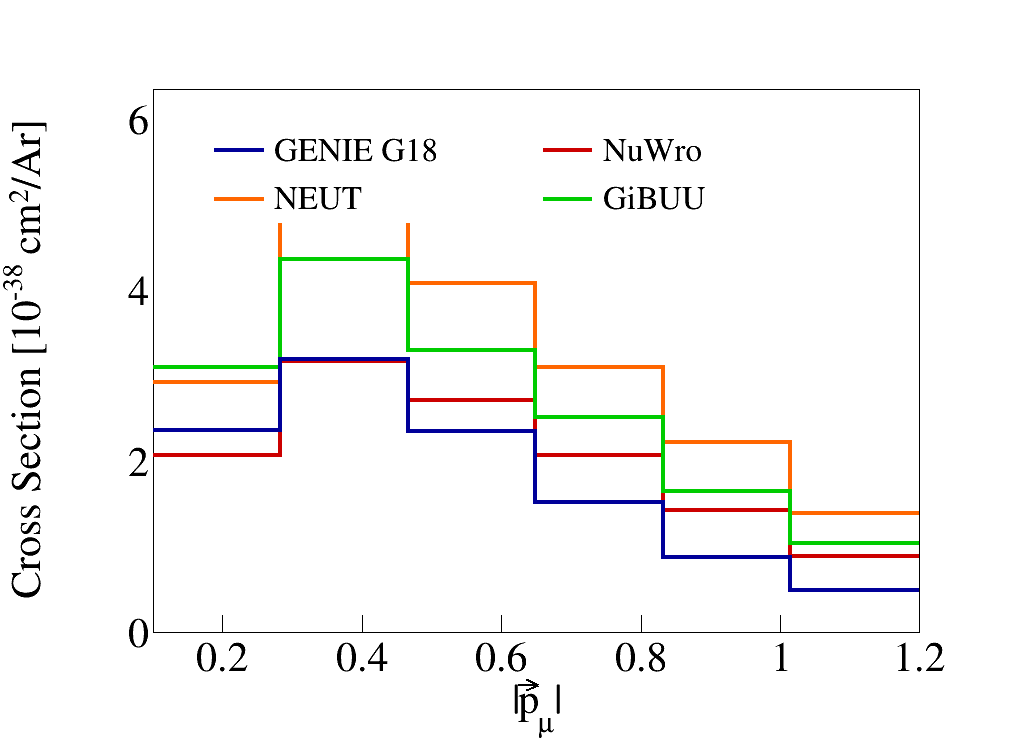
\includegraphics[width=3in]{Figs/Overlay/PostFSI/Overlay_TrueMuonMomentumPlot.png}}
    \subfloat{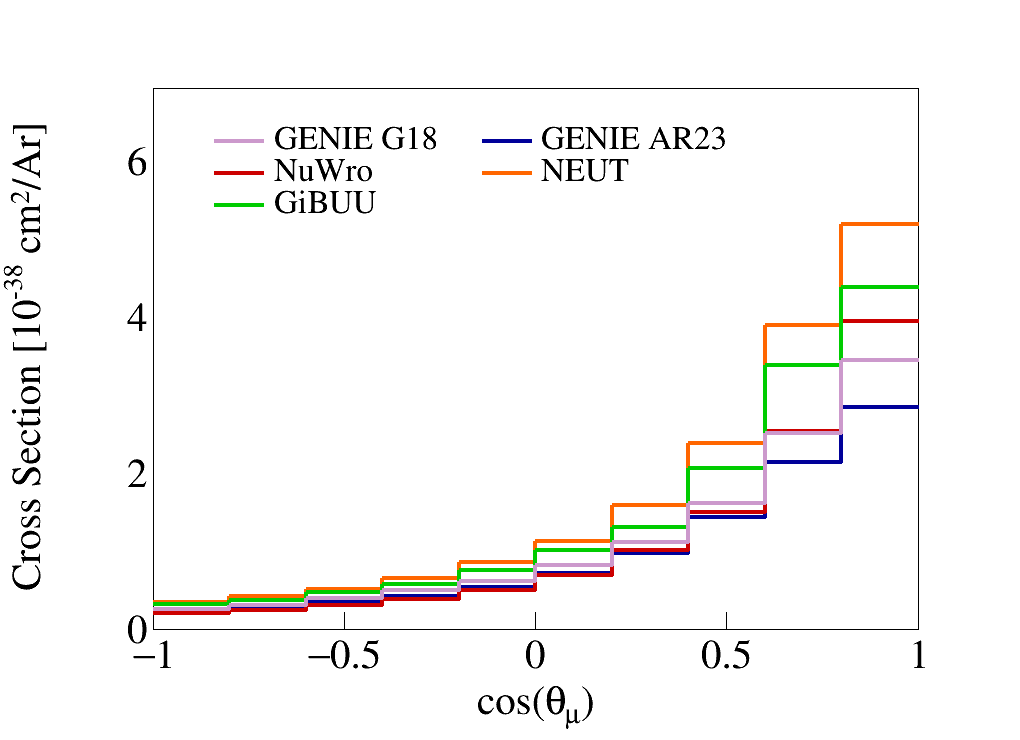
\includegraphics[width=3in]{Figs/Overlay/PostFSI/Overlay_TrueMuonCosThetaPlot.png}} \\
    \subfloat{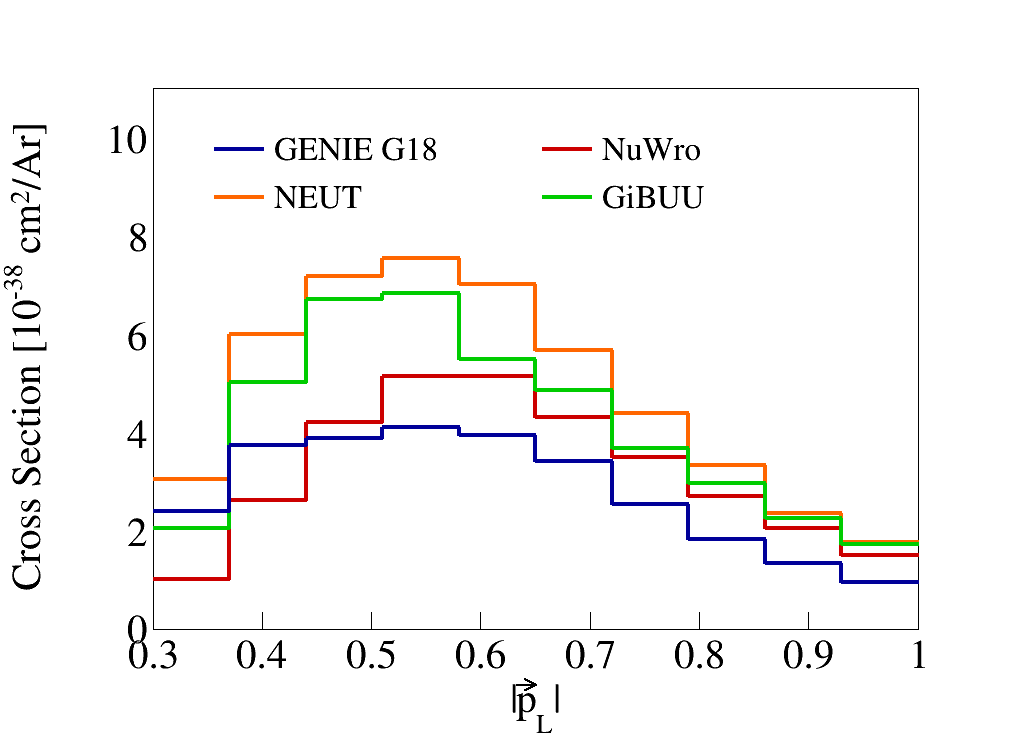
\includegraphics[width=3in]{Figs/Overlay/PostFSI/Overlay_TrueLeadingProtonMomentumPlot.png}}
    \subfloat{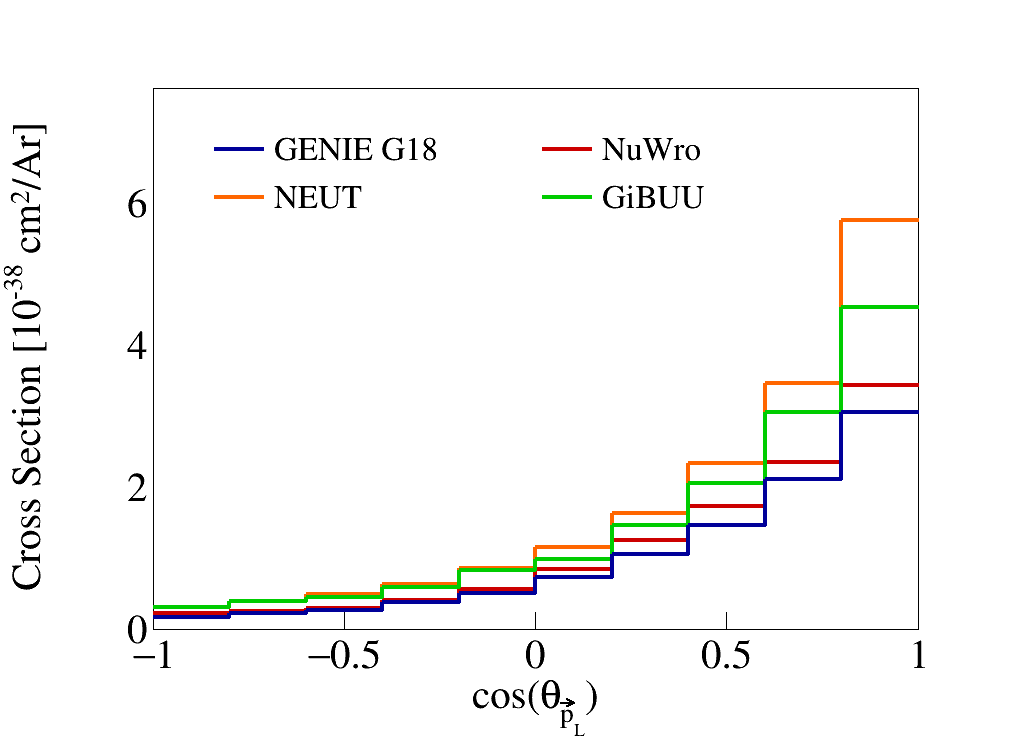
\includegraphics[width=3in]{Figs/Overlay/PostFSI/Overlay_TrueLeadingProtonCosThetaPlot.png}} \\
    \subfloat{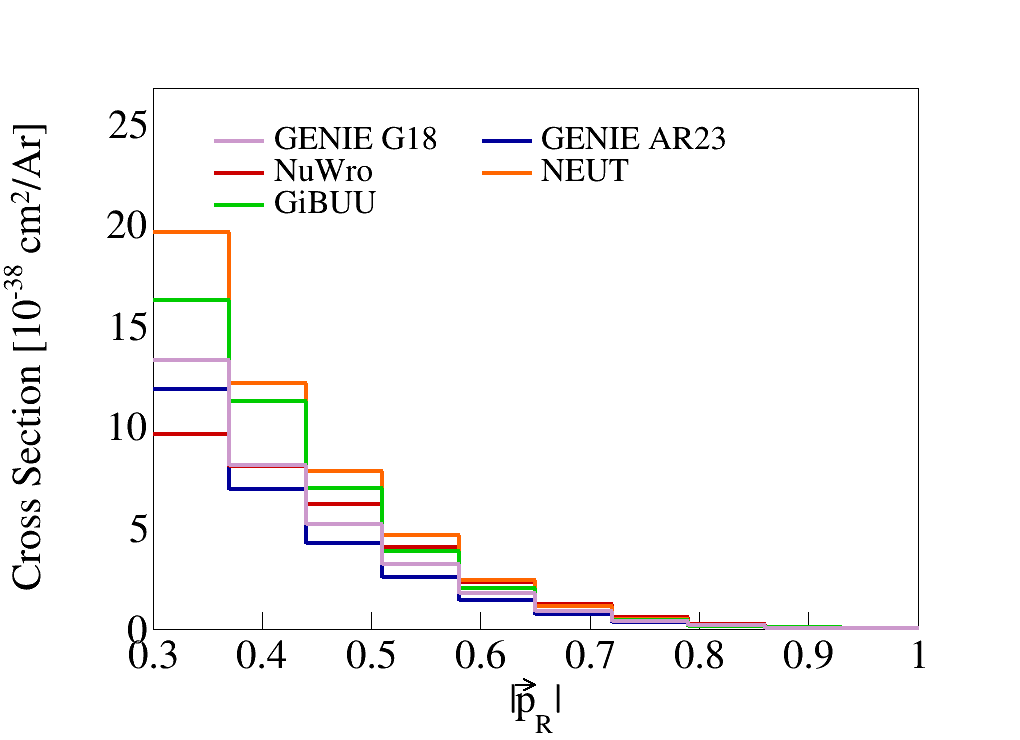
\includegraphics[width=3in]{Figs/Overlay/PostFSI/Overlay_TrueRecoilProtonMomentumPlot.png}}
    \subfloat{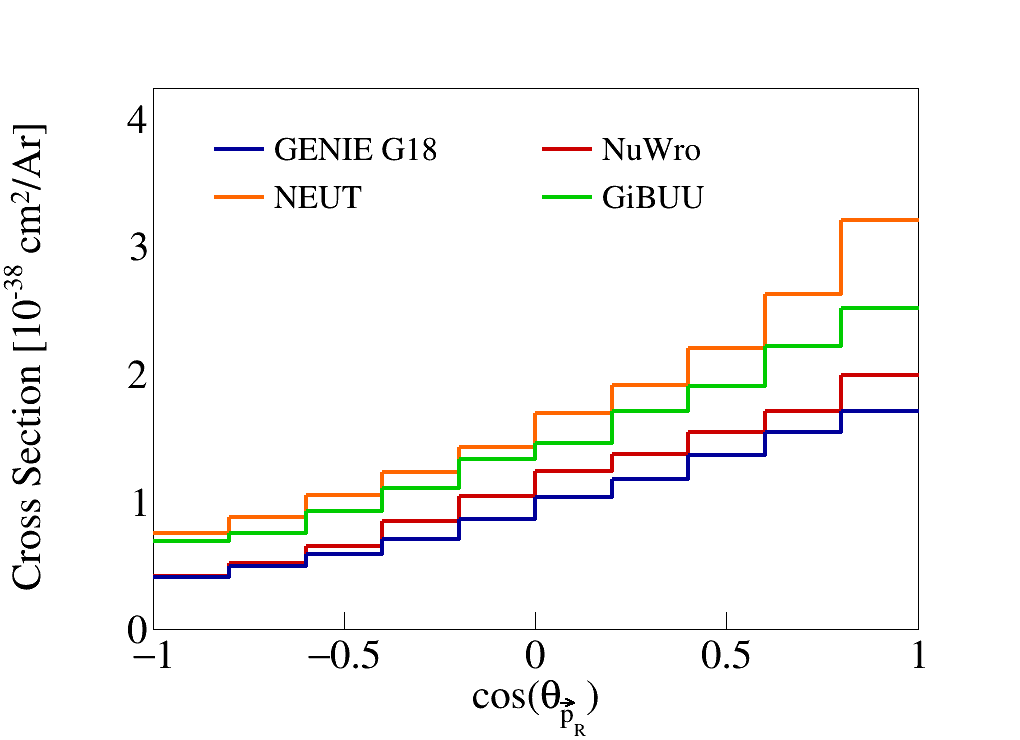
\includegraphics[width=3in]{Figs/Overlay/PostFSI/Overlay_TrueRecoilProtonCosThetaPlot.png}} \\
    \caption{Cross sections for momenta and angles of individual particles}
    \label{fig:momenta-cos-theta}
\end{figure}

We also define variables relating the multiple momentum vectors. First, the opening angle between the protons in the lab frame, given by 
\begin{align}
    \cos\left(\theta_{\vlp,\vrp}\right) = \frac{\vlp \cdot \vrp}{|\vlp||\vrp|}.
\end{align}
Then, the opening angle between the total proton momentum ($\vtp = \vlp + \vrp$) and the muon, given by 
\begin{align}
    \cos\left(\theta_{\vm,\vtp}\right) = \frac{\vm \cdot \vtp}{|\vm||\vtp|}.
\end{align}
Finally, the momentum transverse to the direction of the neutrino beam, which we denote $\vdp$ and is given by 
\begin{align}
    \vdp = \vec{p}^{\mu}_T + \vec{p}^{L}_T + \vec{p}^{R}_T.
\end{align}
For the transverse momentum, we will be interested in its magnitude $|\vdp|$. We plot the differential cross sections of these variables against for the given generators in Figure~\ref{fig:angles-transverse-momentum}. We can also see the cross section by event type for $|\vdp|$ for the NuWro and GENIE AR23 generators in Figure~\ref{fig:inte-breakdown-dpt}.

\begin{figure}
    \centering
    \subfloat{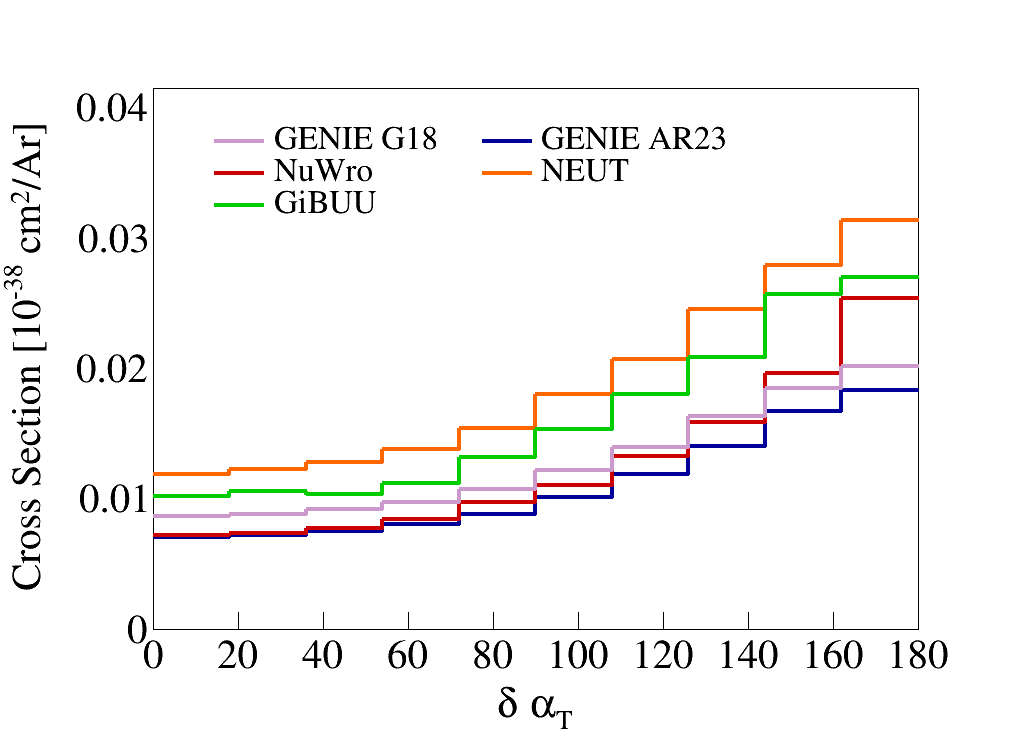
\includegraphics[width=3in]{Figs/Overlay/PostFSI/Overlay_TrueDeltaAlphaTPlot.png}}
    \subfloat{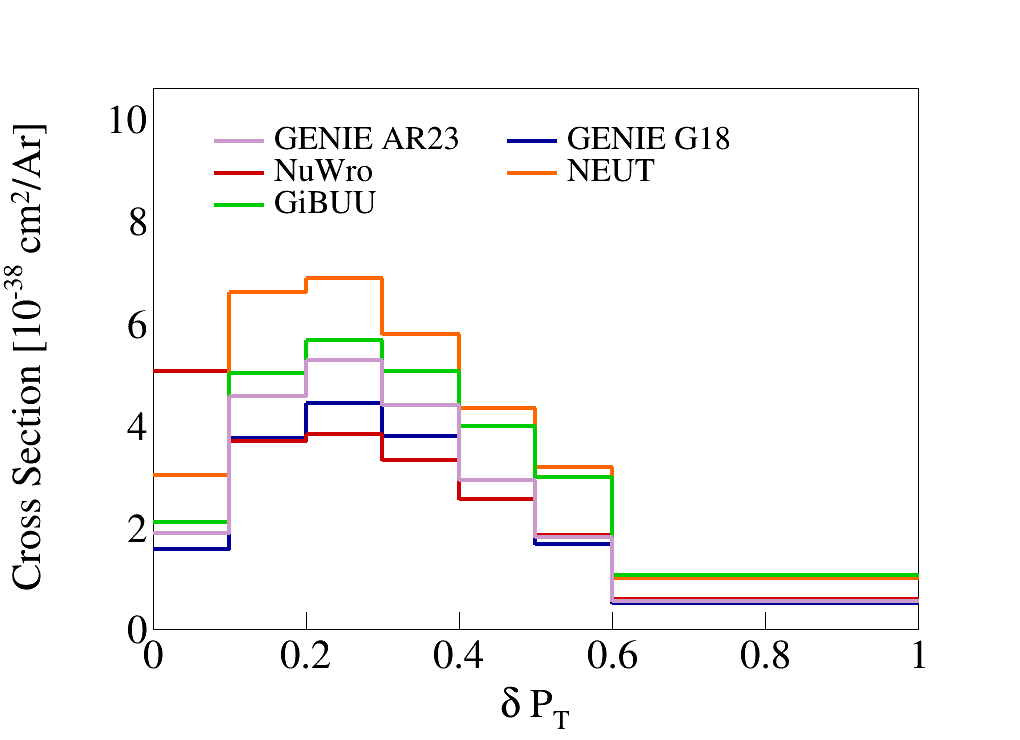
\includegraphics[width=3in]{Figs/Overlay/PostFSI/Overlay_TrueTransverseMomentumPlot.png}} \\
    \subfloat{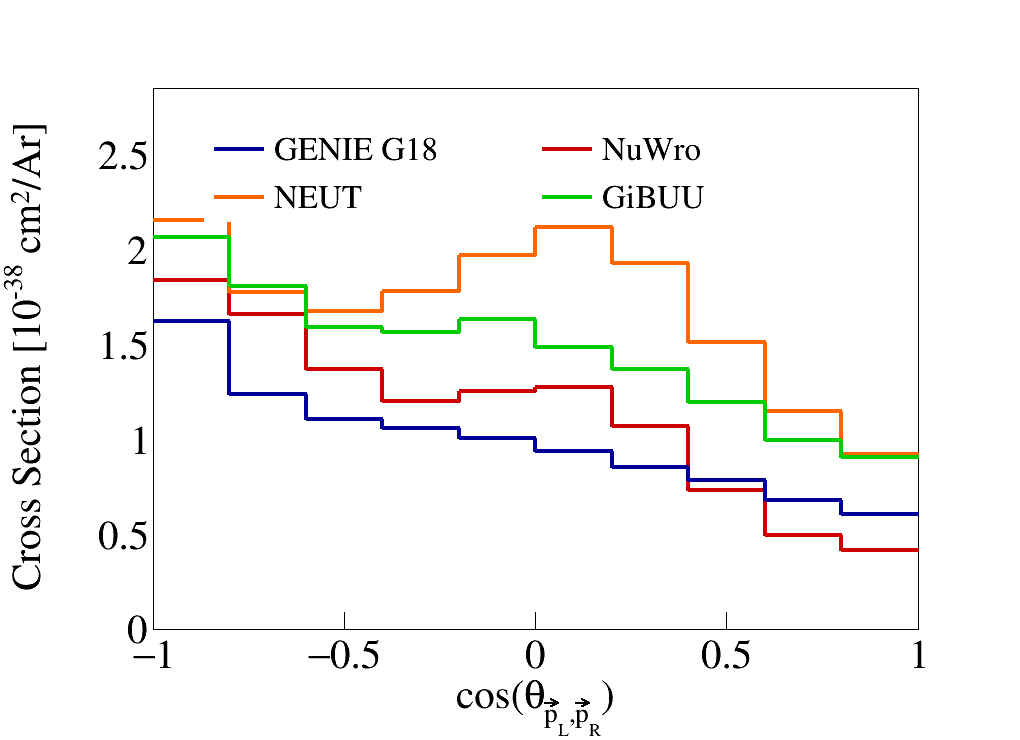
\includegraphics[width=3in]{Figs/Overlay/PostFSI/Overlay_TrueCosOpeningAngleProtonsPlot.png}}
    \subfloat{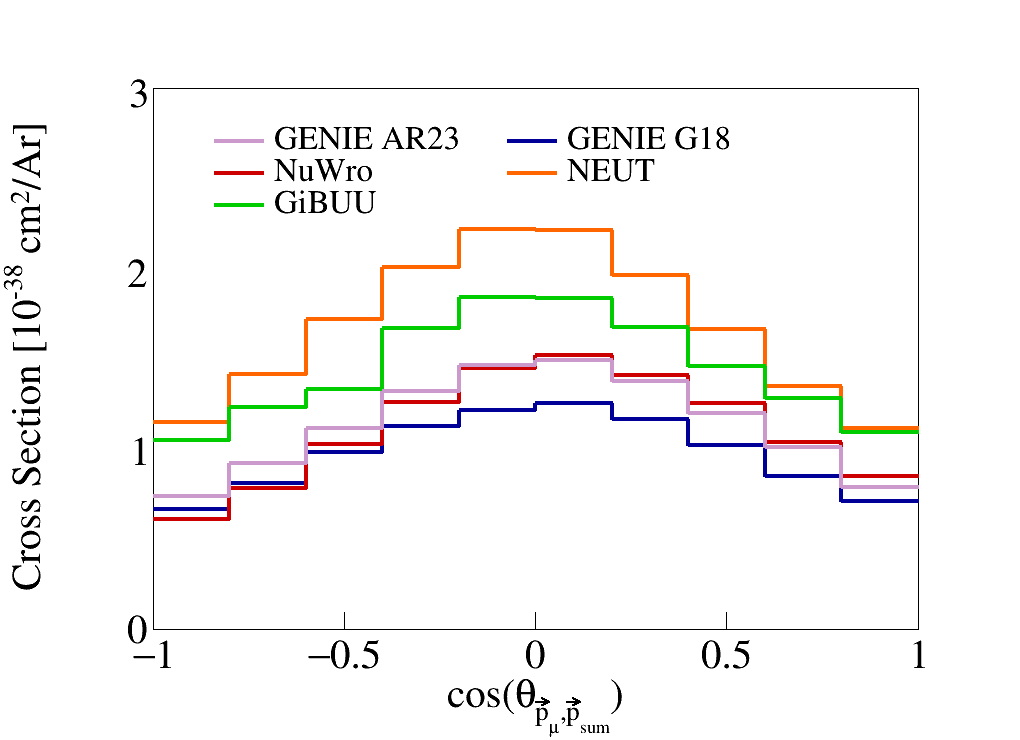
\includegraphics[width=3in]{Figs/Overlay/PostFSI/Overlay_TrueCosOpeningAngleMuonTotalProtonPlot.png}} 
    \caption{Cross sections for opening angles and transverse momentum}
    \label{fig:angles-transverse-momentum}
\end{figure}

\begin{figure}
    \centering
    \subfloat{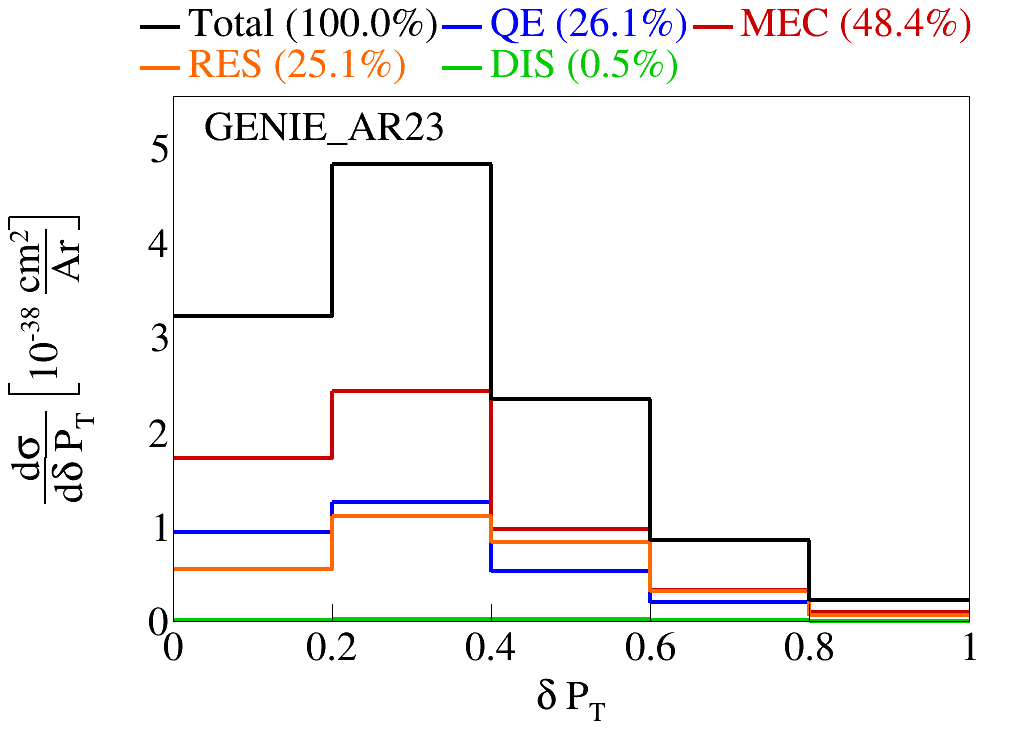
\includegraphics[width=3in]{Figs/InteBreakDown/PostFSI/InteBreakDown_GENIE_AR23_TrueTransverseMomentumPlot.png}}
    \subfloat{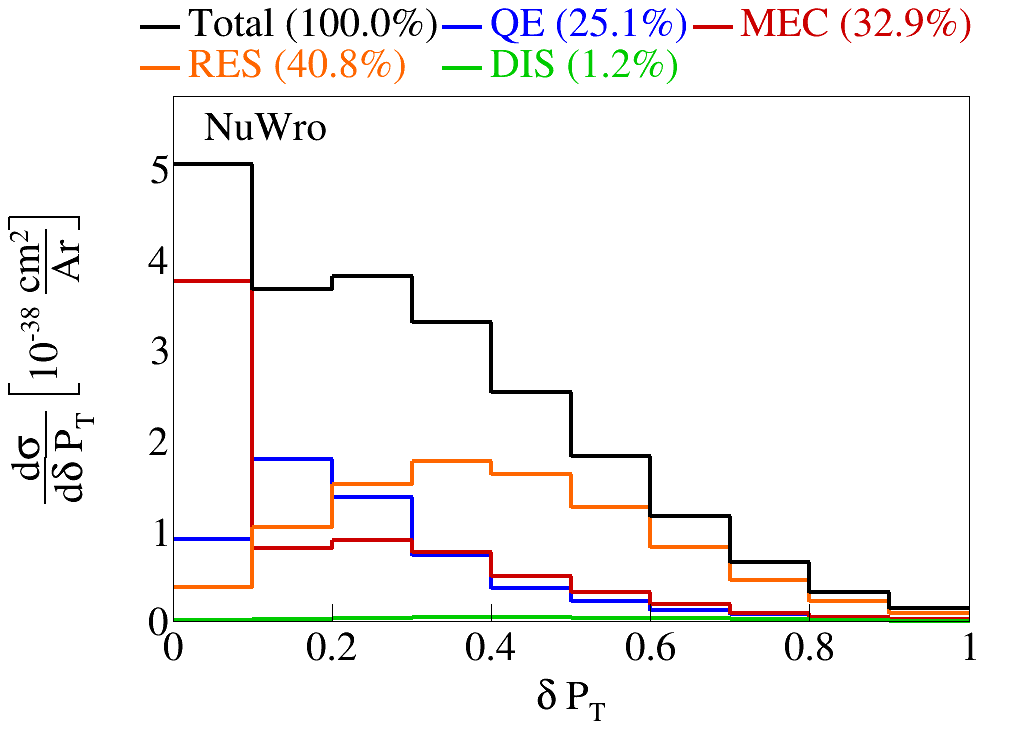
\includegraphics[width=3in]{Figs/InteBreakDown/PostFSI/InteBreakDown_NuWro_TrueTransverseMomentumPlot.png}}
    \caption{Event interaction breakdown for $|\vdp|$}
    \label{fig:inte-breakdown-dpt}
\end{figure}

\section{Pre-FSI events}

To investigate why the percentage of MEC events for some generators is low, we performed event selection before any final state interactions took place. For both GENIE tunes, NEUT, and NuWro, we got 100\% MEC events pre-FSI. For GiBUU, only 4.1\% MEC versus 76.2\% RES and 16\% DIS events pre-FSI. The plots for GiBUU and NuWro are shown in Figure~\ref{fig:pre-fsi-inte-breakdown}. 

Since GiBUU is the outlier, we checked the specific interaction mode for the RES events. We got that 10 has 39.3\%, 11 has 34.7\%, 12 has 0.0136\%, 13 has 26 \%, and 27, 22, and 23 all have zero percent of the RES events. We also checked the event interaction breakdown for GiBUU samples without final state interactions, in which we found that 100\% of the events are MEC, shown in Figure~\ref{fig:gibuu-no-fsi}.

\begin{figure}
    \centering
    \subfloat{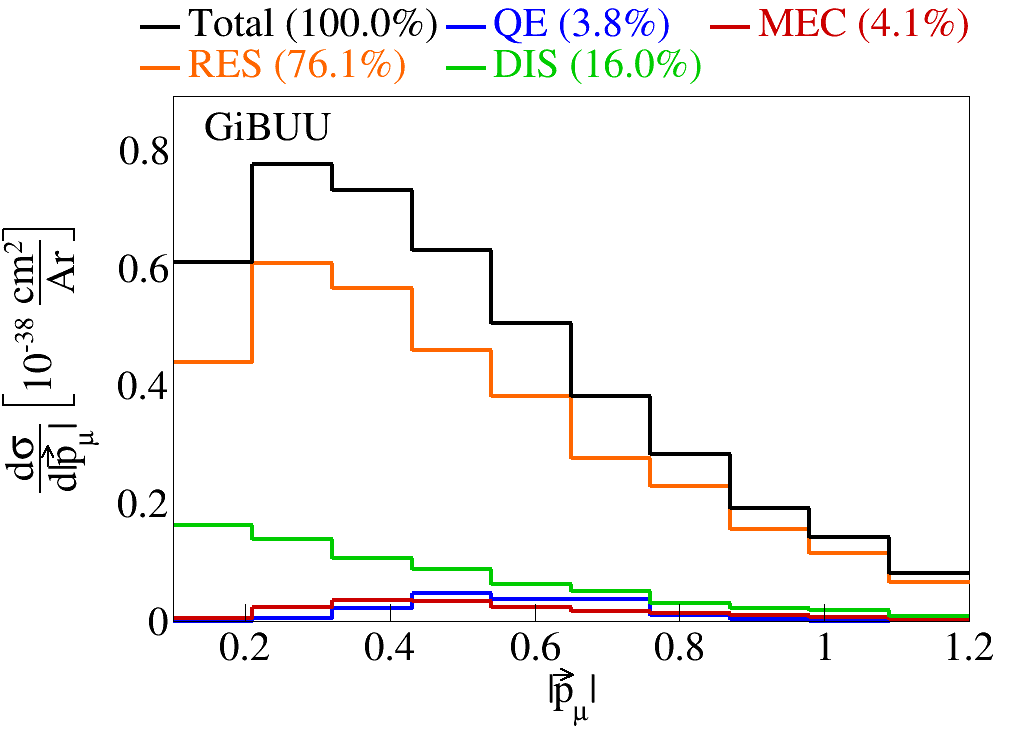
\includegraphics[width=3in]{Figs/InteBreakDown/PreFSI/InteBreakDown_GiBUU_TrueNoFSIMuonMomentumPlot.png}}
    \subfloat{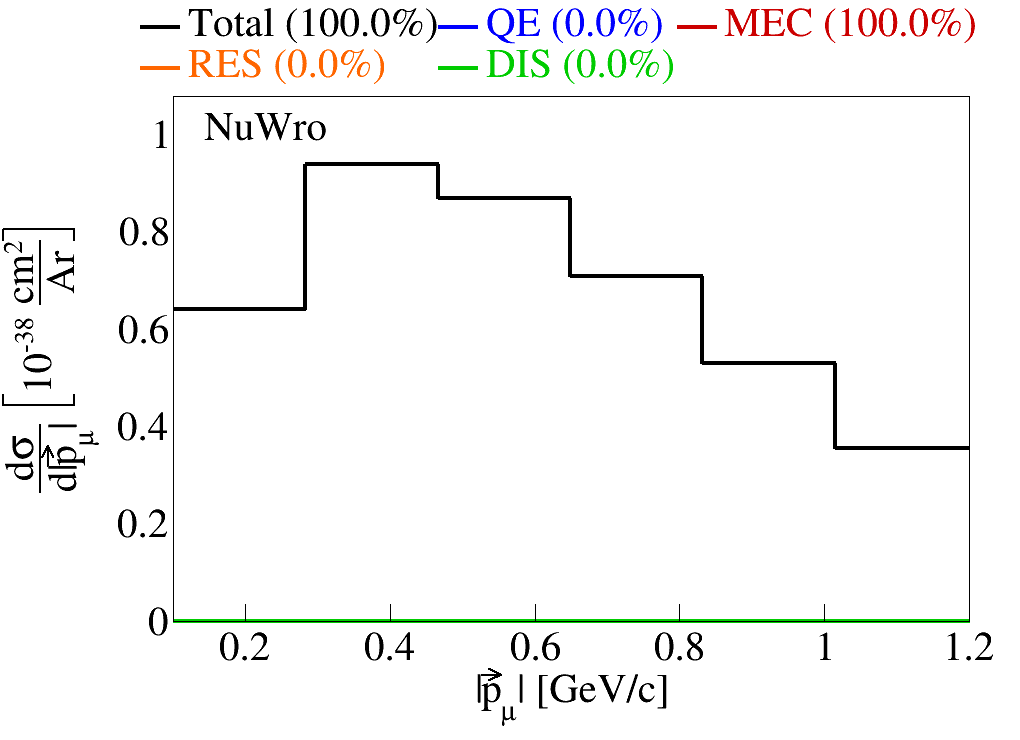
\includegraphics[width=3in]{Figs/InteBreakDown/PreFSI/InteBreakDown_NuWro_TrueNoFSIMuonMomentumPlot.png}}
    \caption{Event interaction breakdown before final state interactions}
    \label{fig:pre-fsi-inte-breakdown}
\end{figure}

\begin{figure}
    \centering
    \subfloat{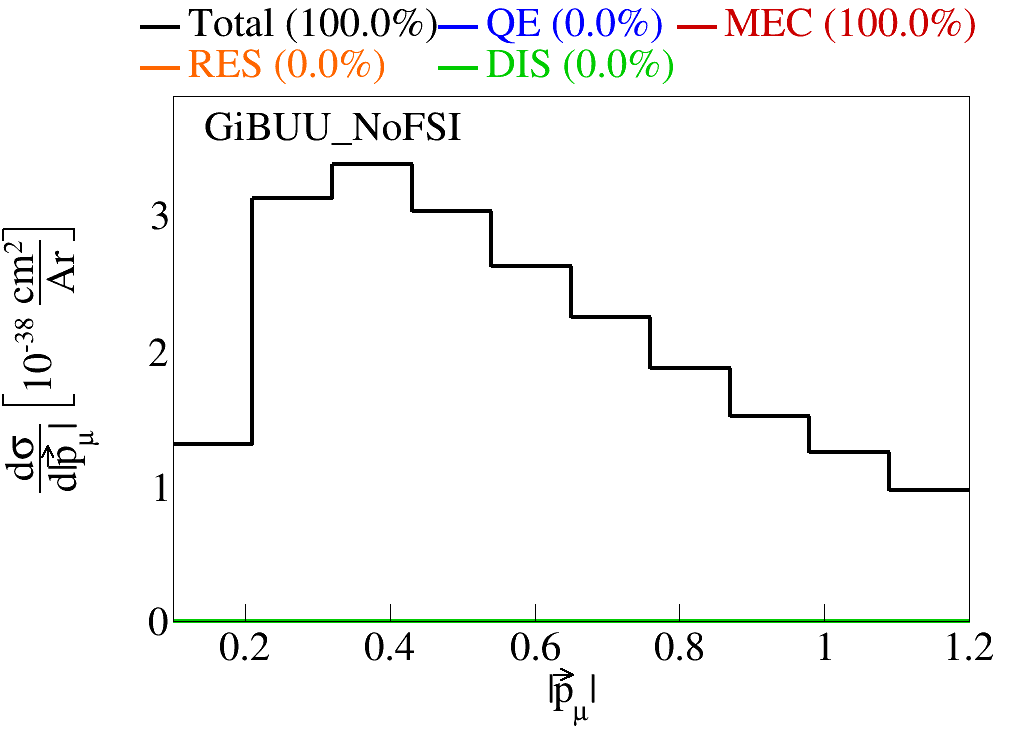
\includegraphics[width=3in]{Figs/InteBreakDown/PostFSI/InteBreakDown_GiBUU_NoFSI_TrueMuonMomentumPlot.png}}
    \caption{Event interaction breakdown for final events from GiBUU events with no FSI}
    \label{fig:gibuu-no-fsi}
\end{figure}

\section{Double differential plots}

We plot $\delta P_T$, $\delta \alpha_T$, $\cos\left(\theta_{\vlp,\vrp}\right)$, and $\cos\left(\theta_{\vm,\vtp}\right)$ in $\cos(\theta_{\vec{p}_{\mu}})$. These are shown in Figure~\ref{fig:double-differential-cos-mu}. We have two bins for $\cos(\theta_{\vec{p}_{\mu}})$, the first one going from $-1$ to $0.5$ and the second from $0.5$ to $1$. Therefore, these are irregular bins, with the first holding a larger range than the first.

\begin{figure}
    \centering
    \subfloat{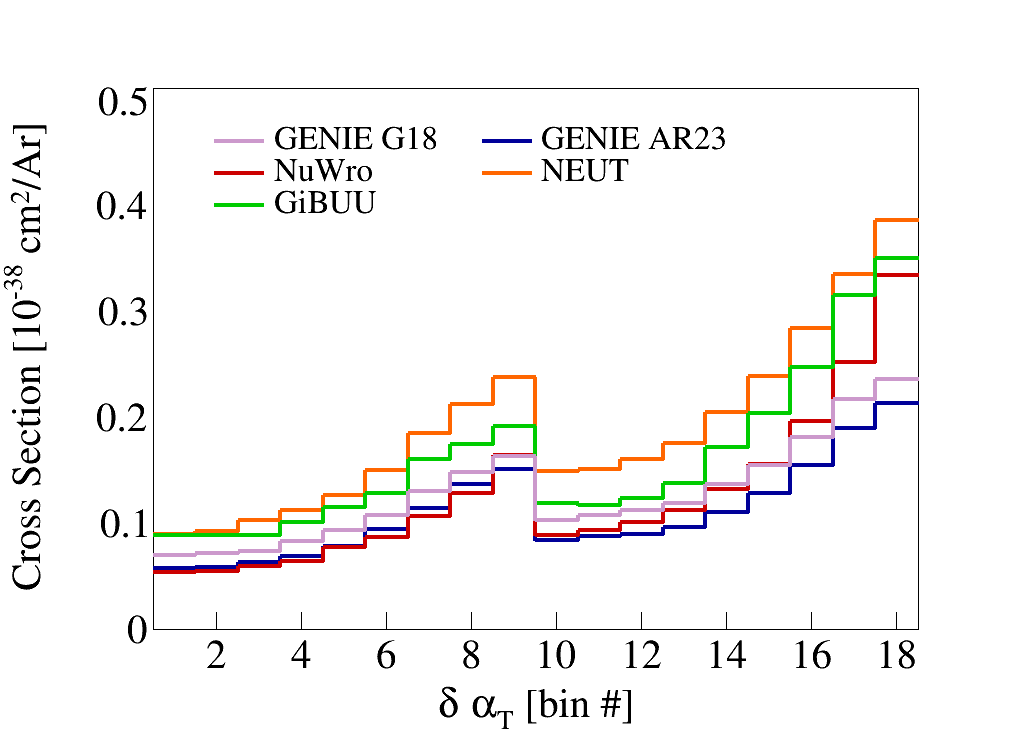
\includegraphics[width=3in]{Figs/Overlay/PostFSI/Overlay_TrueSerialDeltaAlphaT_InMuonCosThetaPlot.png}}
    \subfloat{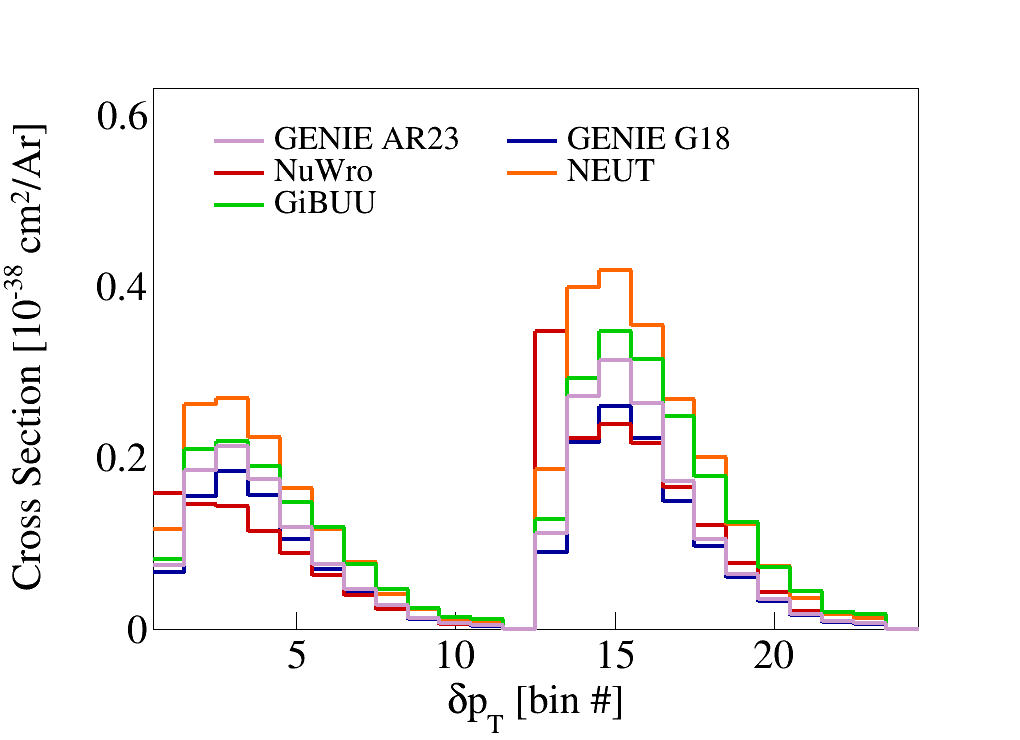
\includegraphics[width=3in]{Figs/Overlay/PostFSI/Overlay_TrueSerialTransverseMomentum_InMuonCosThetaPlot.png}} \\
    \subfloat{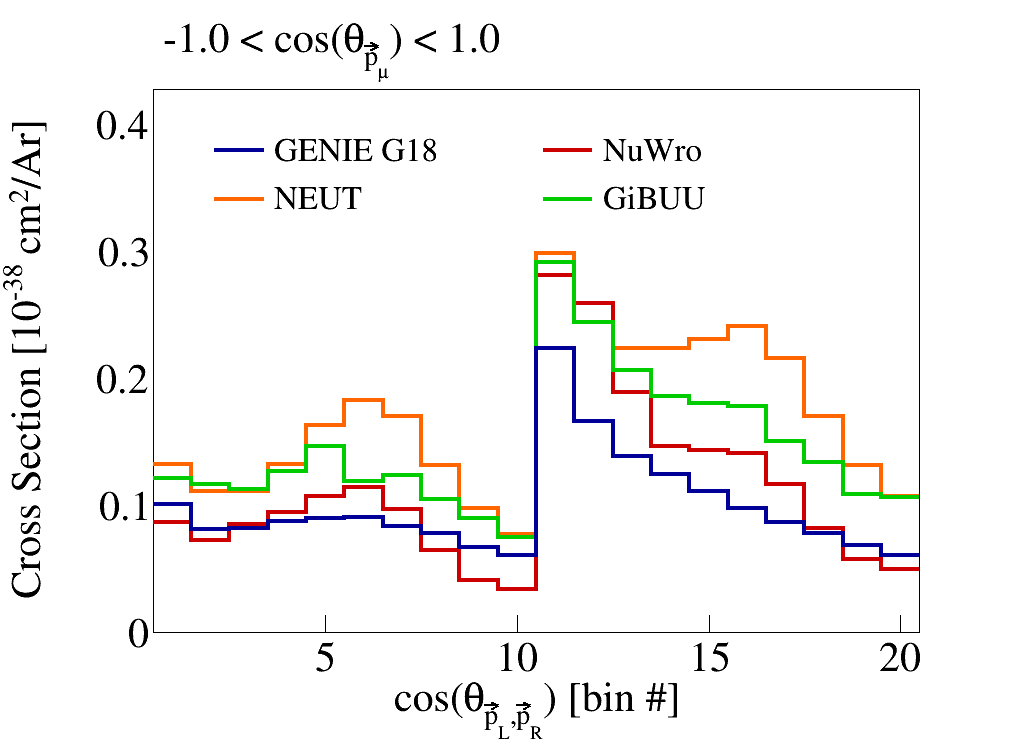
\includegraphics[width=3in]{Figs/Overlay/PostFSI/Overlay_TrueSerialCosOpeningAngleProtons_InMuonCosThetaPlot.png}}
    \subfloat{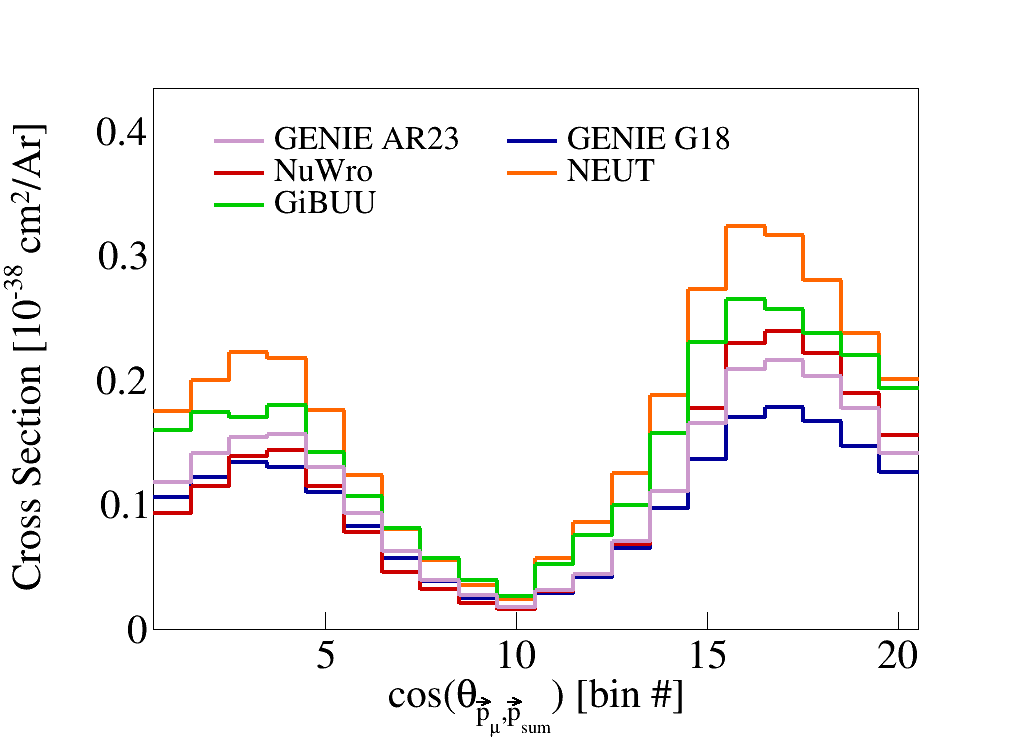
\includegraphics[width=3in]{Figs/Overlay/PostFSI/Overlay_TrueSerialCosOpeningAngleMuonTotalProton_InMuonCosThetaPlot.png}}
    \caption{Double differential serial plots, all in $\cos(\theta_{\vec{p}_{\mu}})$}
    \label{fig:double-differential-cos-mu}
\end{figure}

We also slice the double differential plots into two plots each, so that we have $\cos(\theta_{\vec{p}_{\mu}})$ in the horizontal axis instead of bin numbers. These plots are shown in Figure~\ref{fig:sliced-double-differential-cos-mu}. In these plots, the bins contents have been reweighed appropriately, by dividing the content of each bin by the width of the bin for the variable in the axis multiplied by the width of the $\cos(\theta_{\vec{p}_{\mu}})$ slice. Note that the plots for the $1 < \cos(\theta_{\vec{p}_{\mu}}) < 1.5$ slice have more events in general, as it can be seen by the scale of the vertical axis. 

\begin{figure}
    \centering
    \subfloat{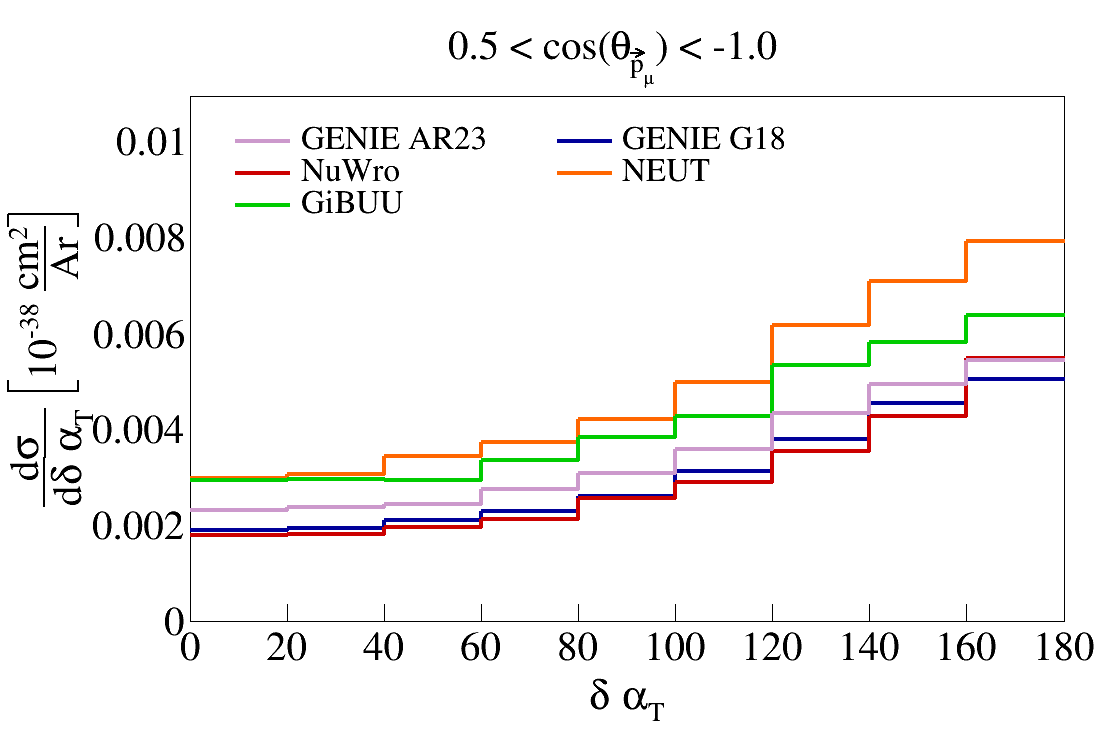
\includegraphics[width=3in]{Figs/Overlay/Serial/TrueSerialDeltaAlphaT_InMuonCosThetaPlot_0.png}}
    \subfloat{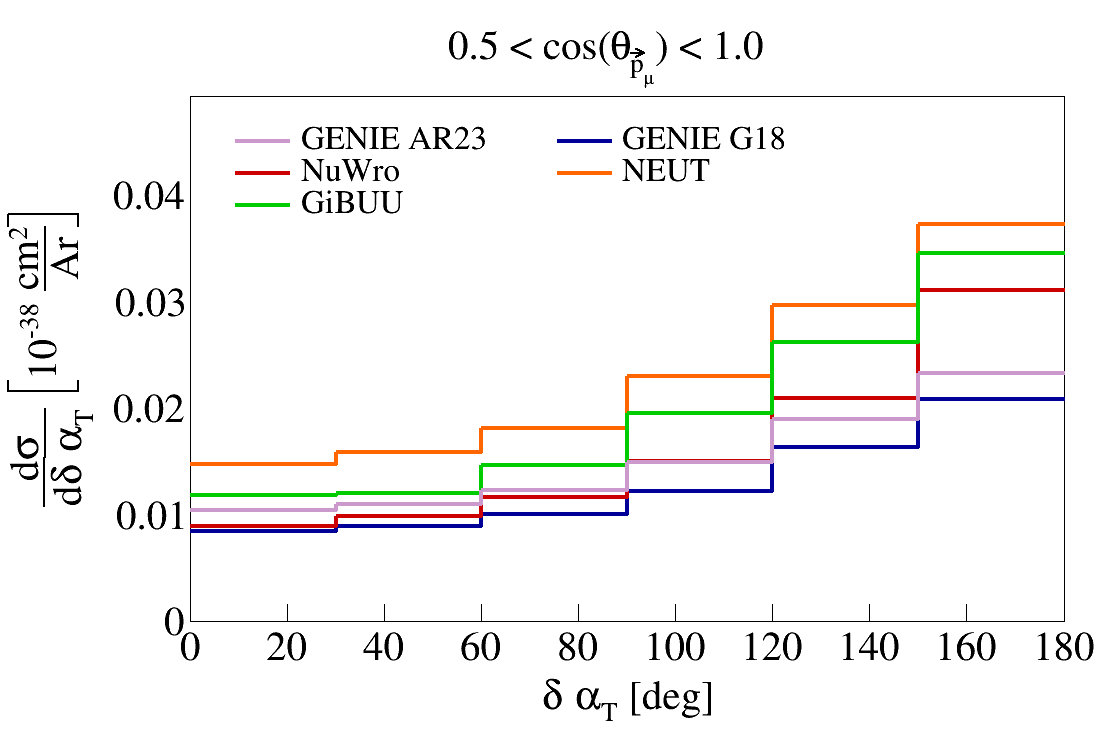
\includegraphics[width=3in]{Figs/Overlay/Serial/TrueSerialDeltaAlphaT_InMuonCosThetaPlot_1.png}} \\
    \subfloat{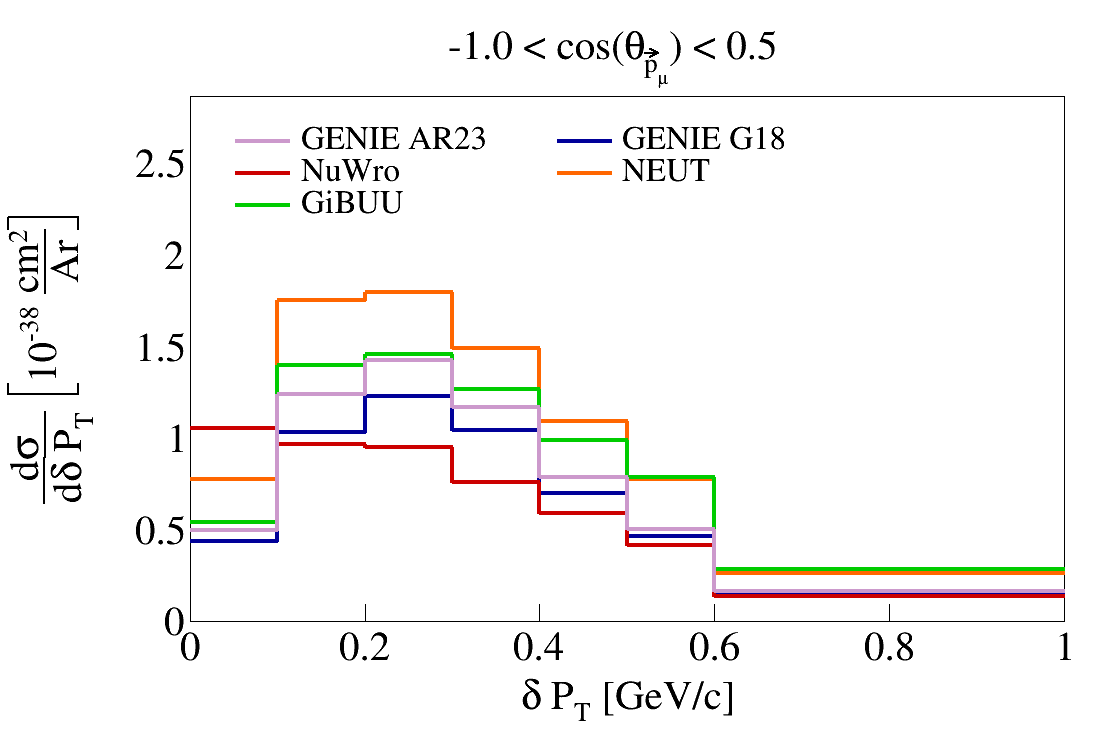
\includegraphics[width=3in]{Figs/Overlay/Serial/TrueSerialTransverseMomentum_InMuonCosThetaPlot_0.png}}
    \subfloat{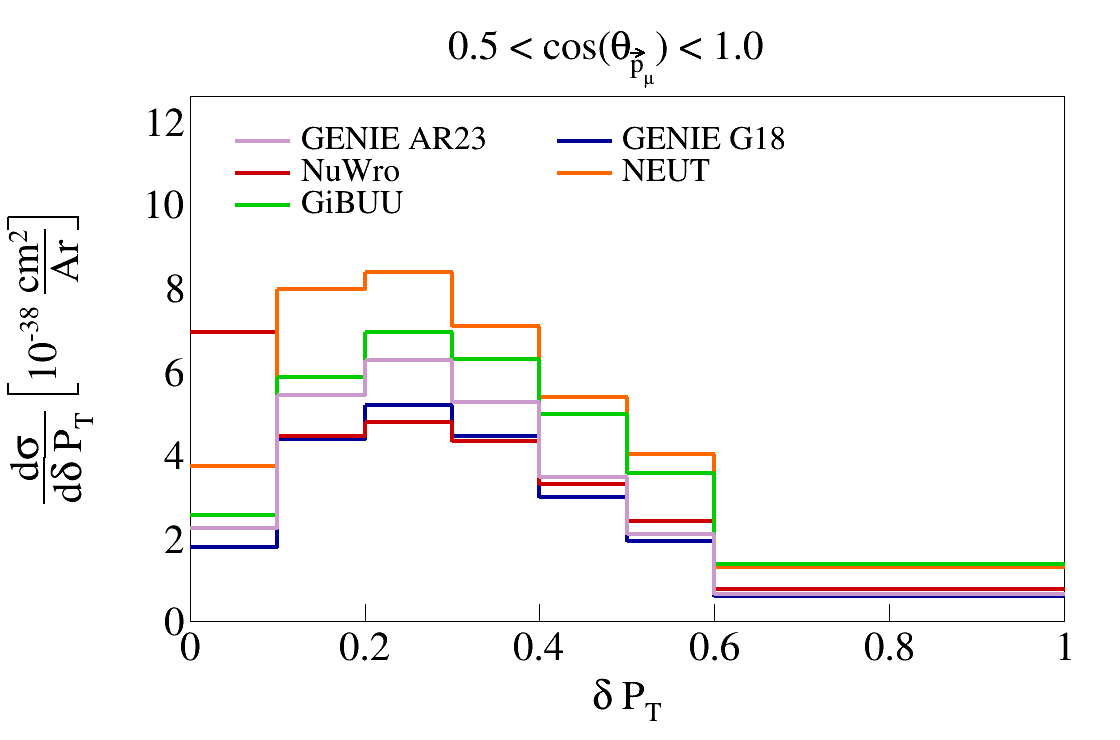
\includegraphics[width=3in]{Figs/Overlay/Serial/TrueSerialTransverseMomentum_InMuonCosThetaPlot_1.png}} \\
    \subfloat{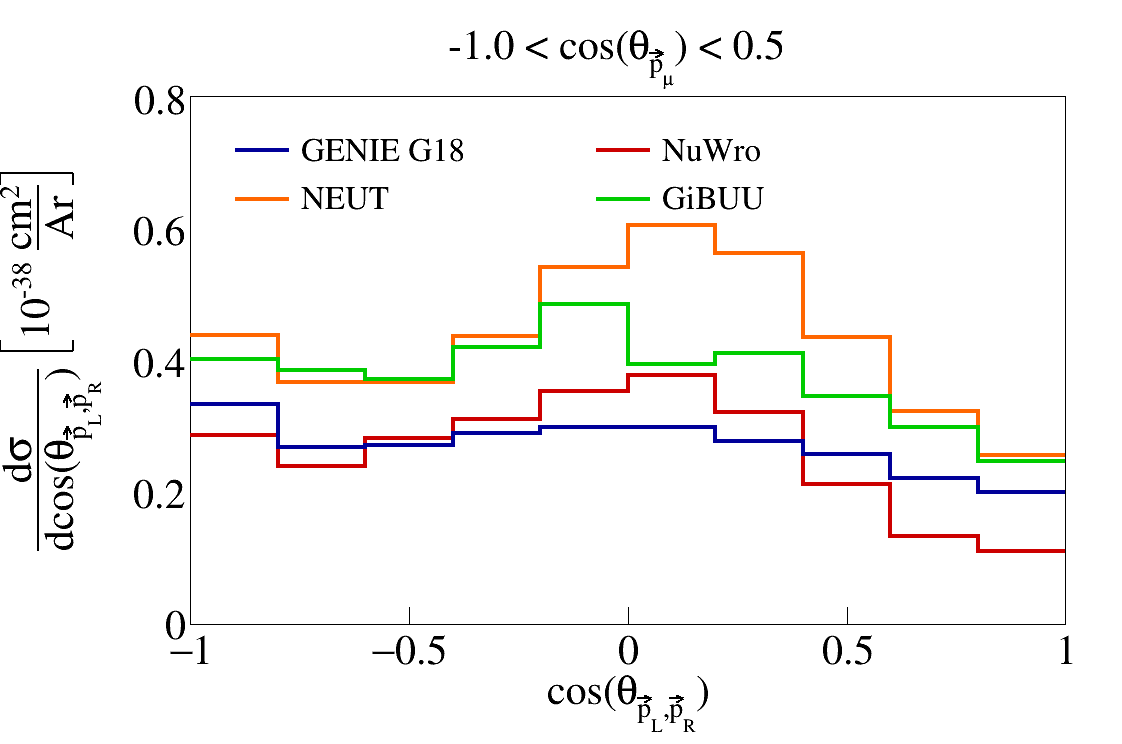
\includegraphics[width=3in]{Figs/Overlay/Serial/TrueSerialCosOpeningAngleProtons_InMuonCosThetaPlot_0.png}}
    \subfloat{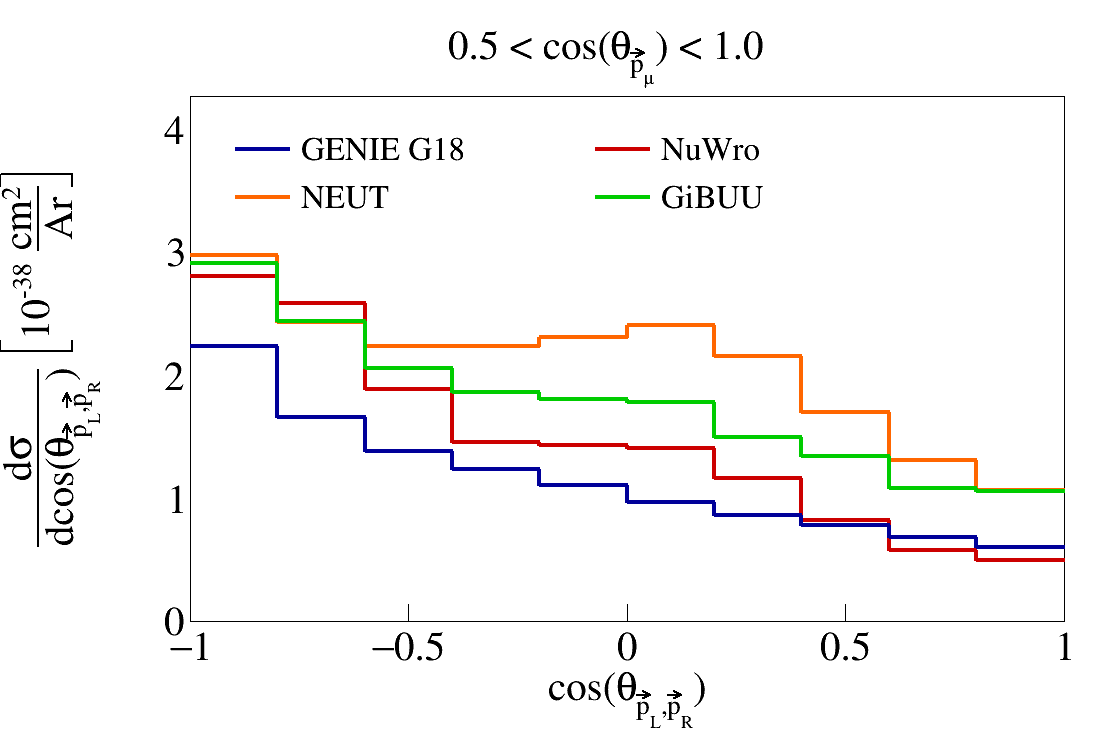
\includegraphics[width=3in]{Figs/Overlay/Serial/TrueSerialCosOpeningAngleProtons_InMuonCosThetaPlot_1.png}} \\
    \subfloat{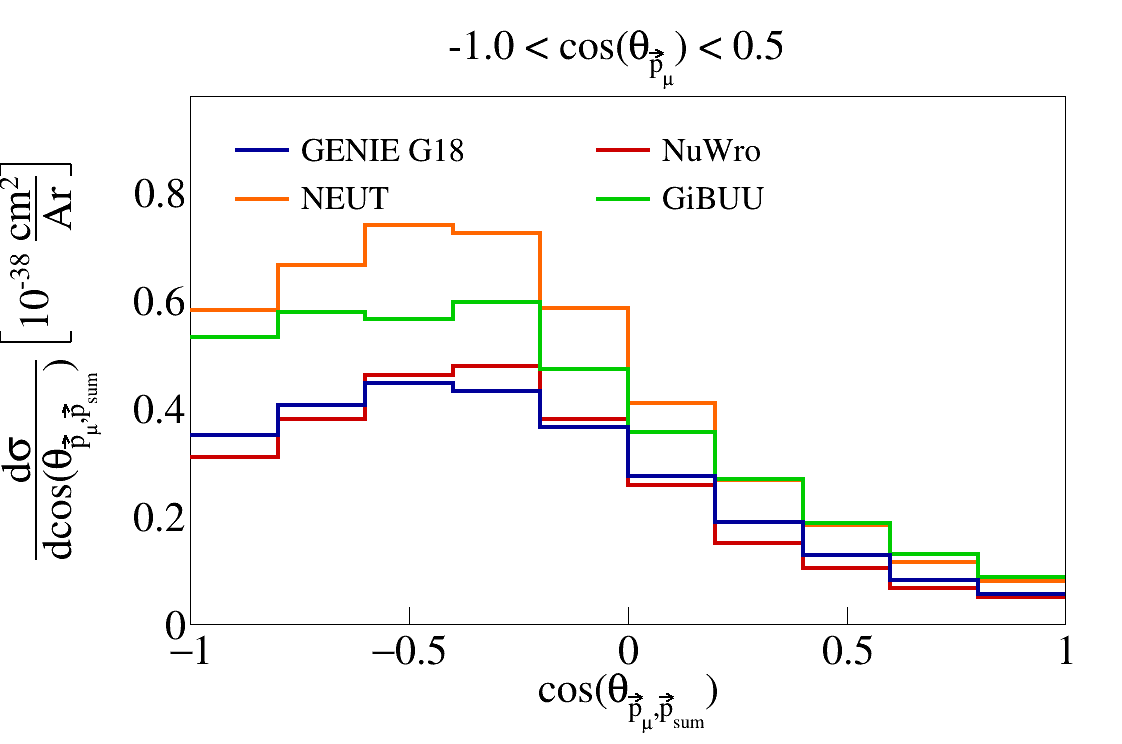
\includegraphics[width=3in]{Figs/Overlay/Serial/TrueSerialCosOpeningAngleMuonTotalProton_InMuonCosThetaPlot_0.png}}
    \subfloat{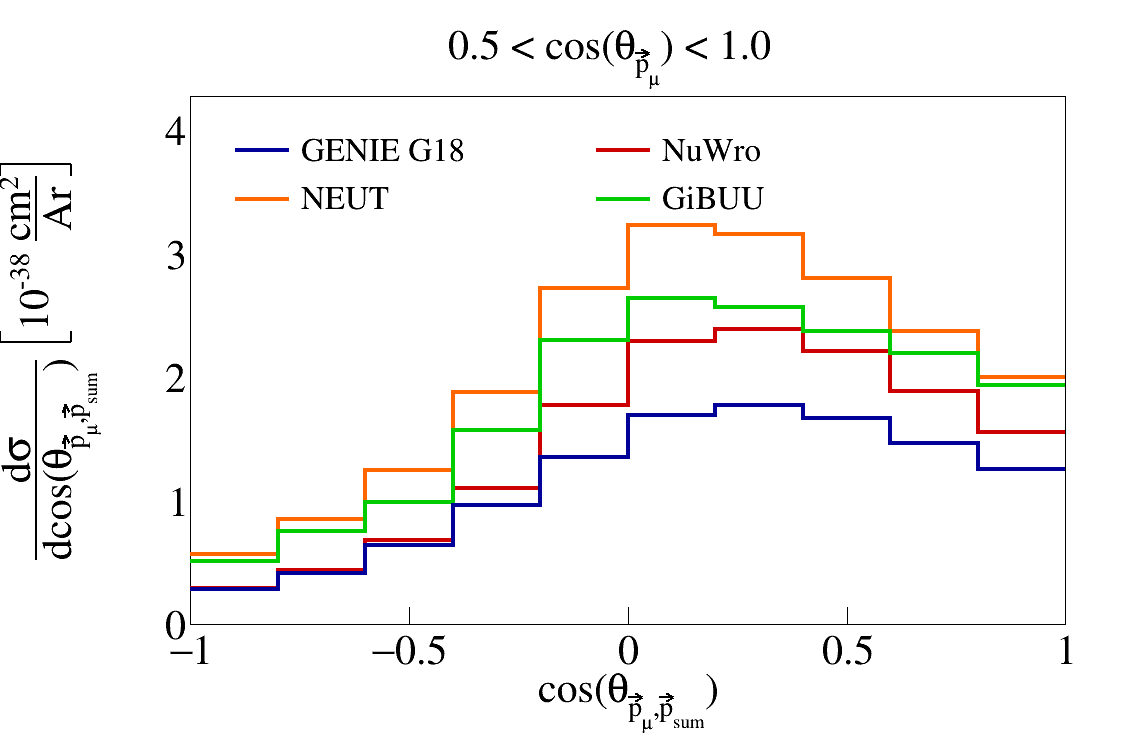
\includegraphics[width=3in]{Figs/Overlay/Serial/TrueSerialCosOpeningAngleMuonTotalProton_InMuonCosThetaPlot_1.png}} 
    \caption{Sliced double differential plots}
    \label{fig:sliced-double-differential-cos-mu}
\end{figure}

We also performed the same double differential analysis but for the events before final state interactions. These are shown in Figure~\ref{fig:sliced-double-differential-cos-mu-no-fsi}. Only the plots for the two opening angles are shown here for compactness. 

\begin{figure}
    \centering
    % \subfloat{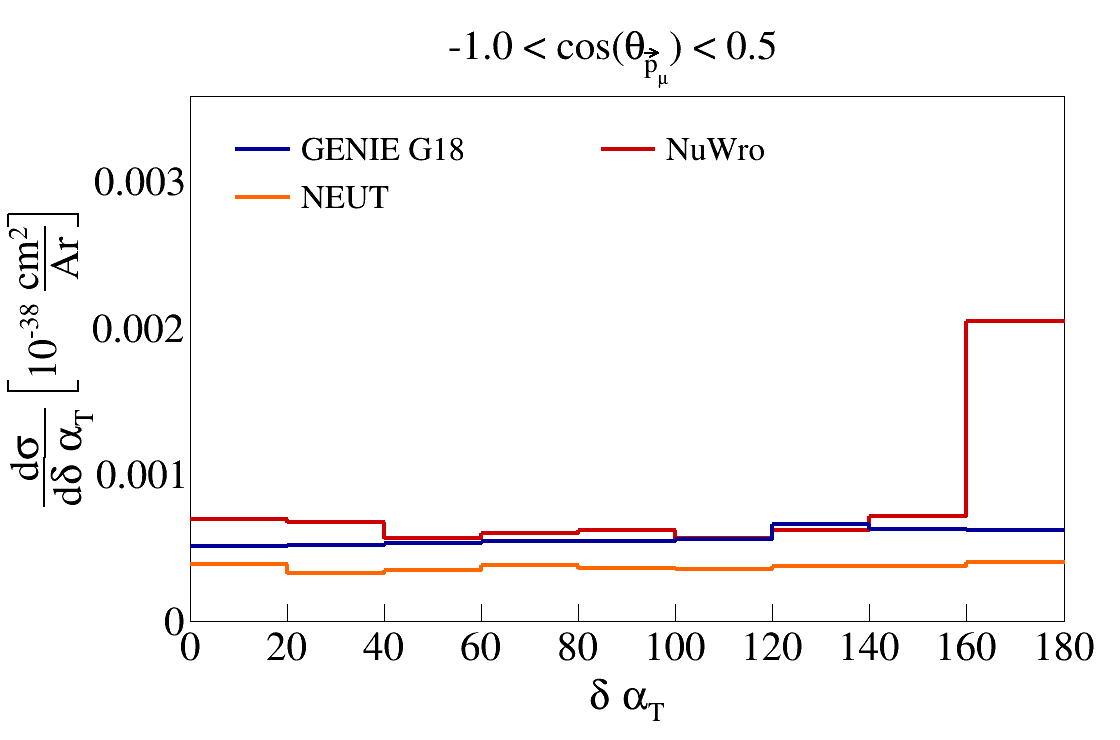
\includegraphics[width=3in]{Figs/Overlay/Serial/TrueSerialNoFSIDeltaAlphaT_InMuonCosThetaPlot_0.png}}
    % \subfloat{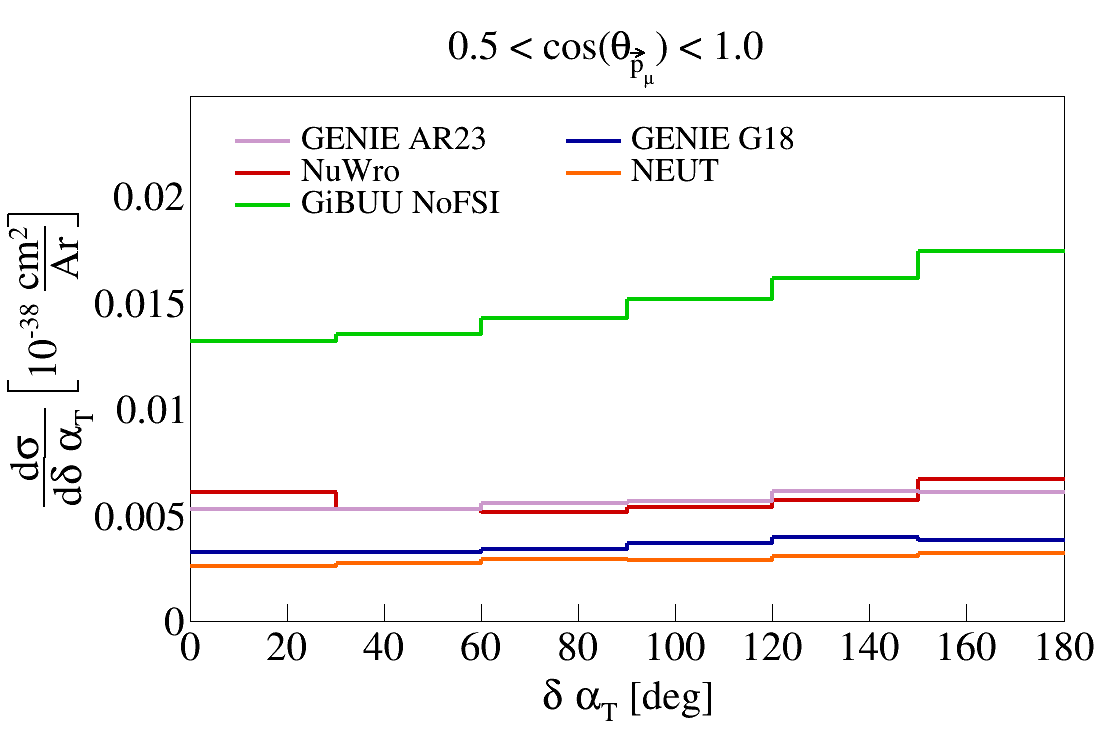
\includegraphics[width=3in]{Figs/Overlay/Serial/TrueSerialNoFSIDeltaAlphaT_InMuonCosThetaPlot_1.png}} \\
    % \subfloat{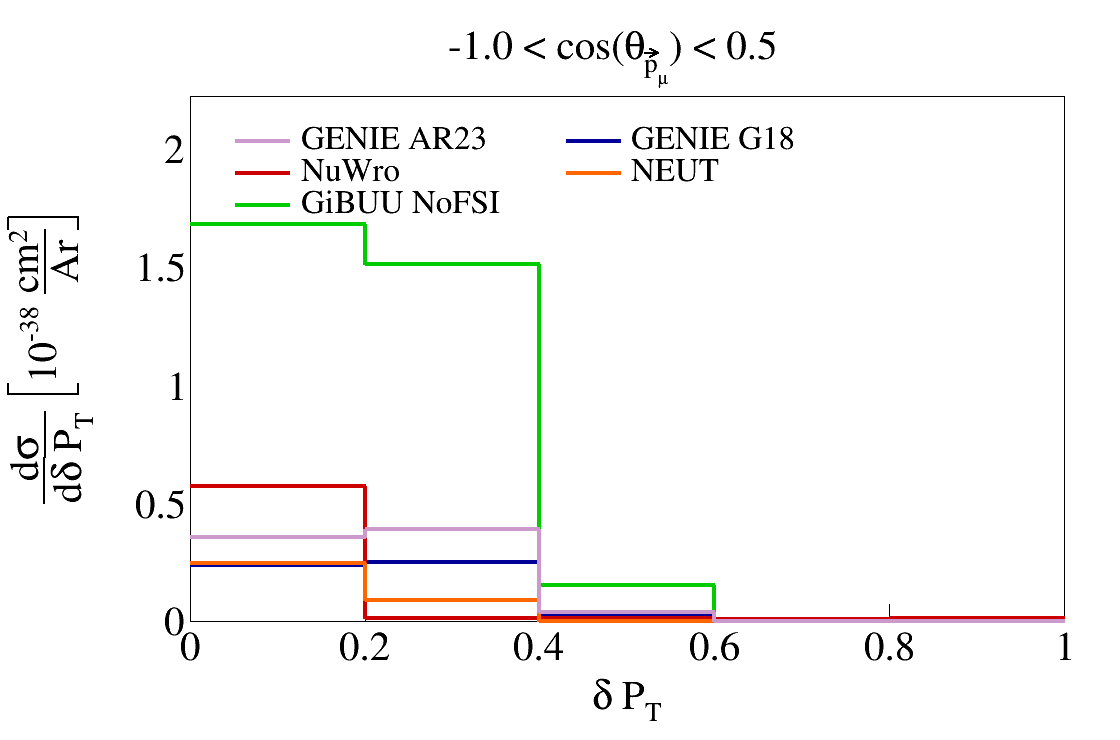
\includegraphics[width=3in]{Figs/Overlay/Serial/TrueSerialNoFSITransverseMomentum_InMuonCosThetaPlot_0.png}}
    % \subfloat{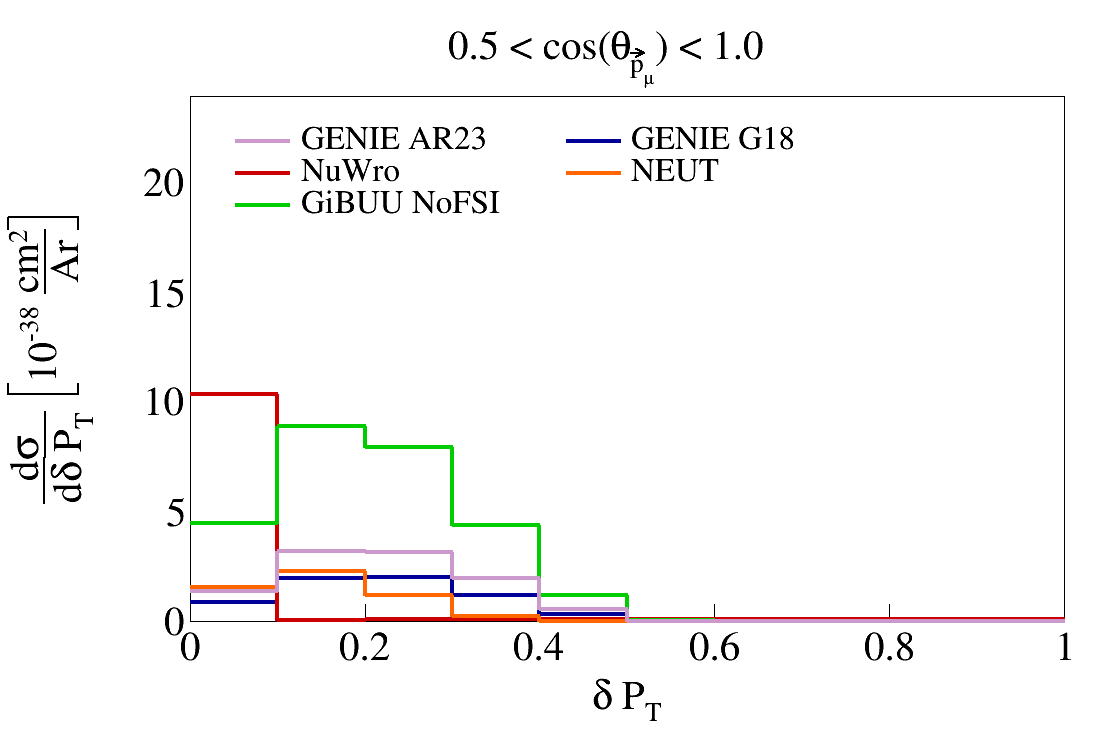
\includegraphics[width=3in]{Figs/Overlay/Serial/TrueSerialNoFSITransverseMomentum_InMuonCosThetaPlot_1.png}} \\
    \subfloat{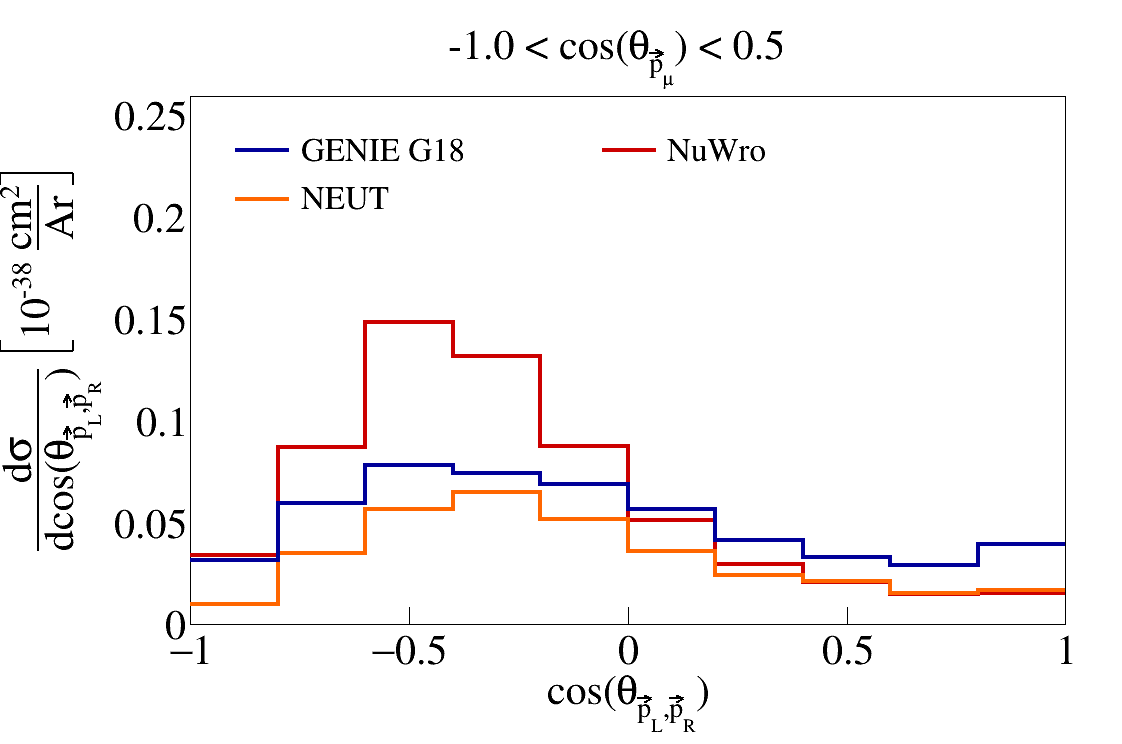
\includegraphics[width=3in]{Figs/Overlay/Serial/TrueSerialNoFSICosOpeningAngleProtons_InMuonCosThetaPlot_0.png}}
    \subfloat{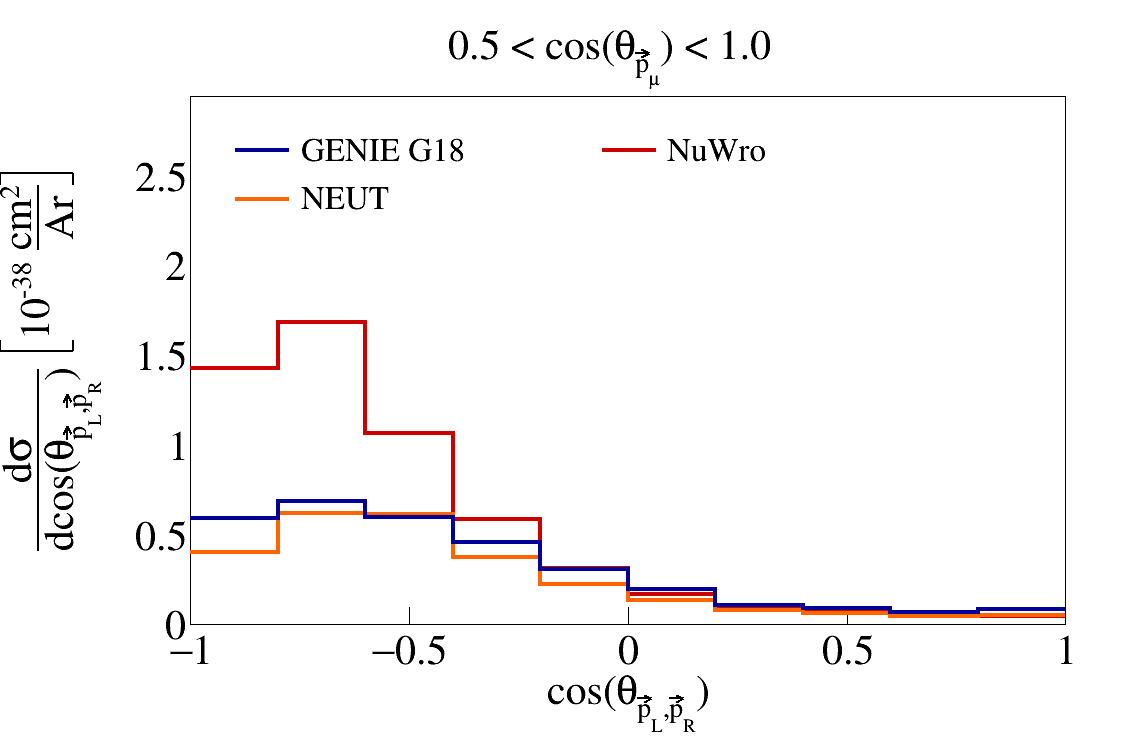
\includegraphics[width=3in]{Figs/Overlay/Serial/TrueSerialNoFSICosOpeningAngleProtons_InMuonCosThetaPlot_1.png}} \\
    \subfloat{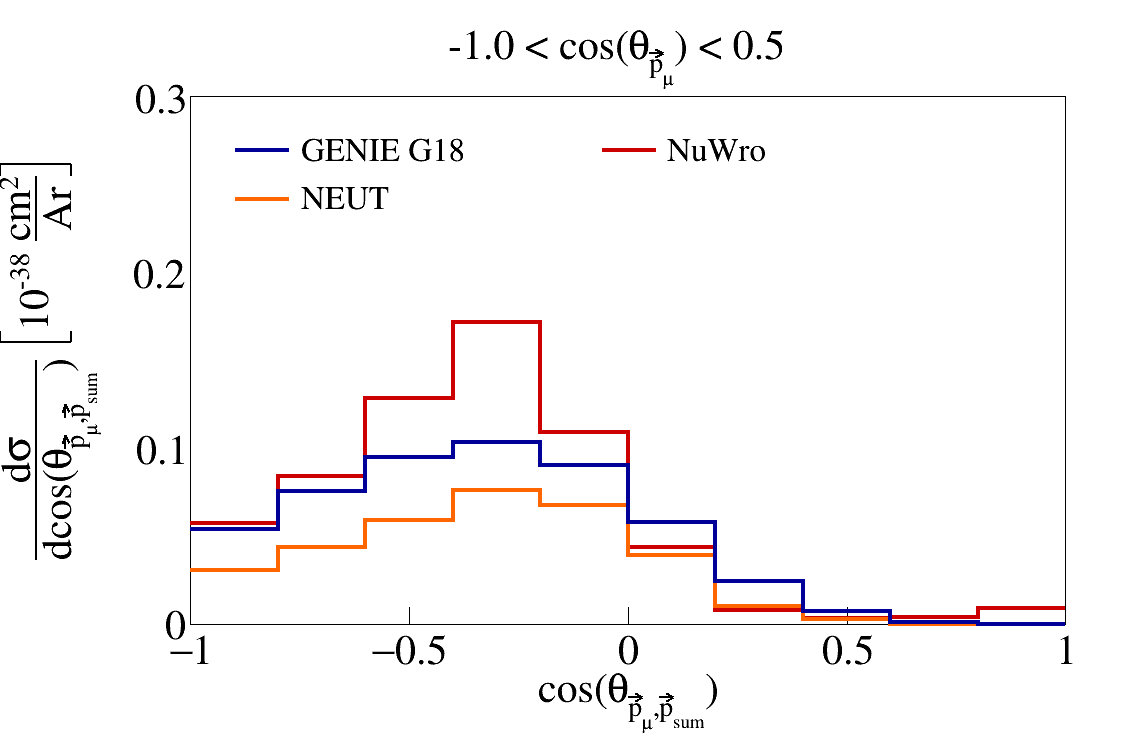
\includegraphics[width=3in]{Figs/Overlay/Serial/TrueSerialNoFSICosOpeningAngleMuonTotalProton_InMuonCosThetaPlot_0.png}}
    \subfloat{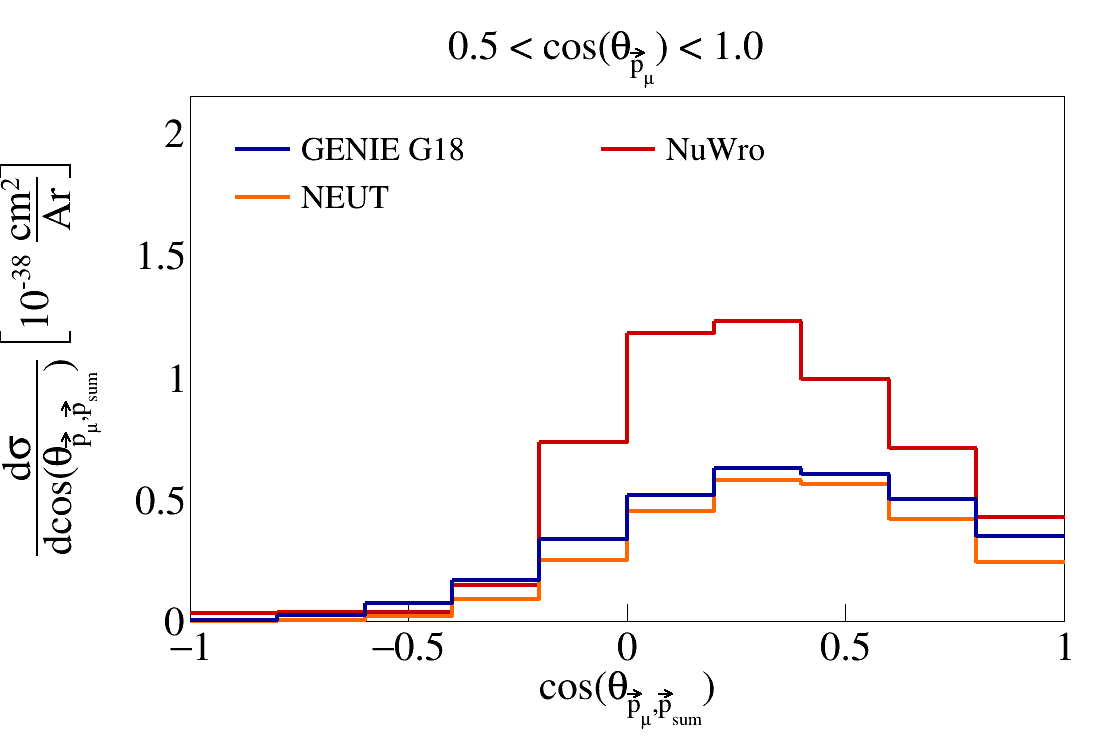
\includegraphics[width=3in]{Figs/Overlay/Serial/TrueSerialNoFSICosOpeningAngleMuonTotalProton_InMuonCosThetaPlot_1.png}} 
    \caption{Sliced double differential plots for pre-FSI events}
    \label{fig:sliced-double-differential-cos-mu-no-fsi}
\end{figure}

\section{Pure MEC events}

We also generated pure MEC events with different configurations to get the MEC splines. These were all different tunes of GENIE: AR23, G18 with Empirical MEC model, and G18 with Nieves MEC model. The plots for the transverse kinematic variables are shown in Figure~\ref{fig:transverse-k-mec}. Some of the sliced double differential plots are shown in Figure~\ref{fig:sliced-double-mec}.

\begin{figure}
    \centering
    \subfloat{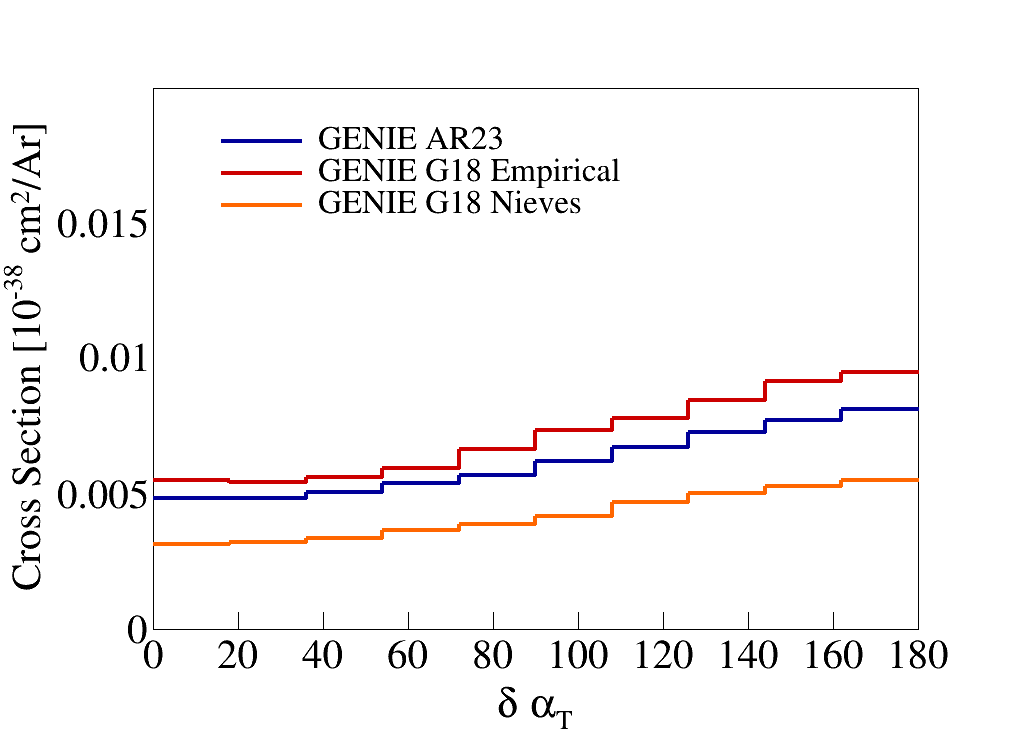
\includegraphics[width=3in]{Figs/Overlay/MEC/Overlay_TrueDeltaAlphaTPlot.png}}
    \subfloat{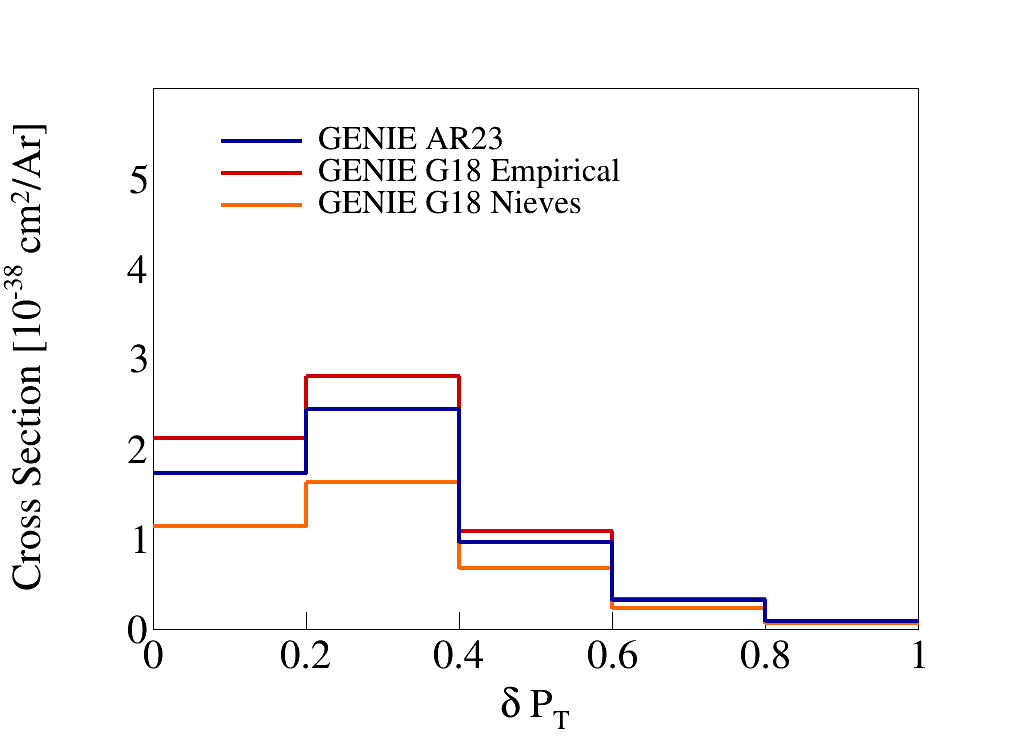
\includegraphics[width=3in]{Figs/Overlay/MEC/Overlay_TrueTransverseMomentumPlot.png}} \\
    \subfloat{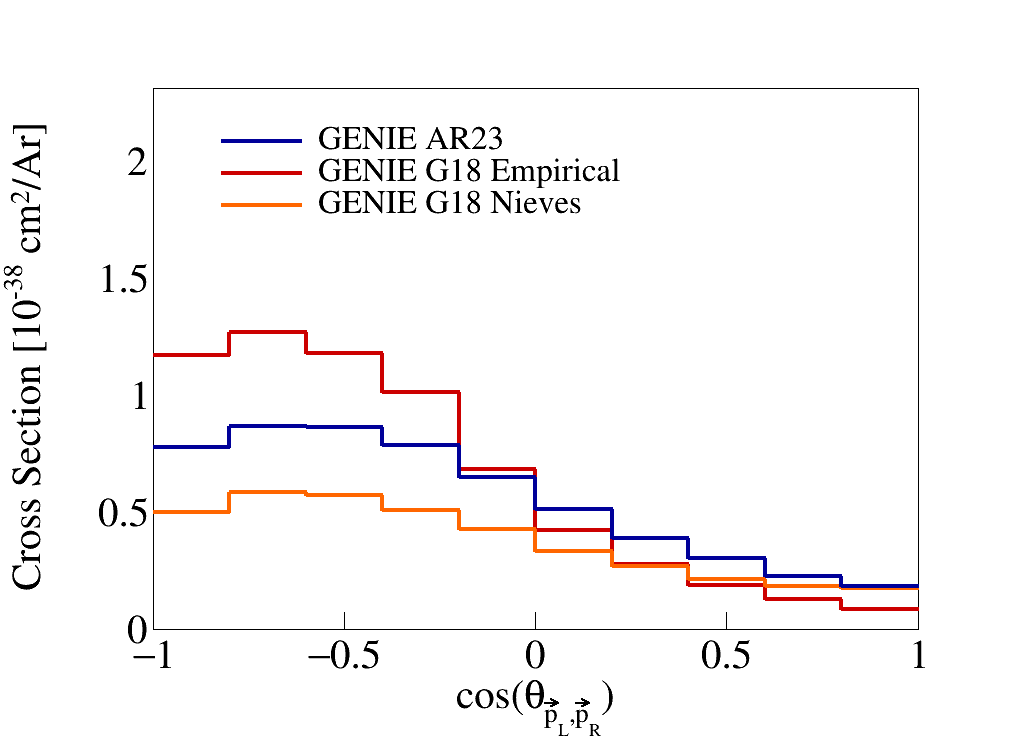
\includegraphics[width=3in]{Figs/Overlay/MEC/Overlay_TrueCosOpeningAngleProtonsPlot.png}}
    \subfloat{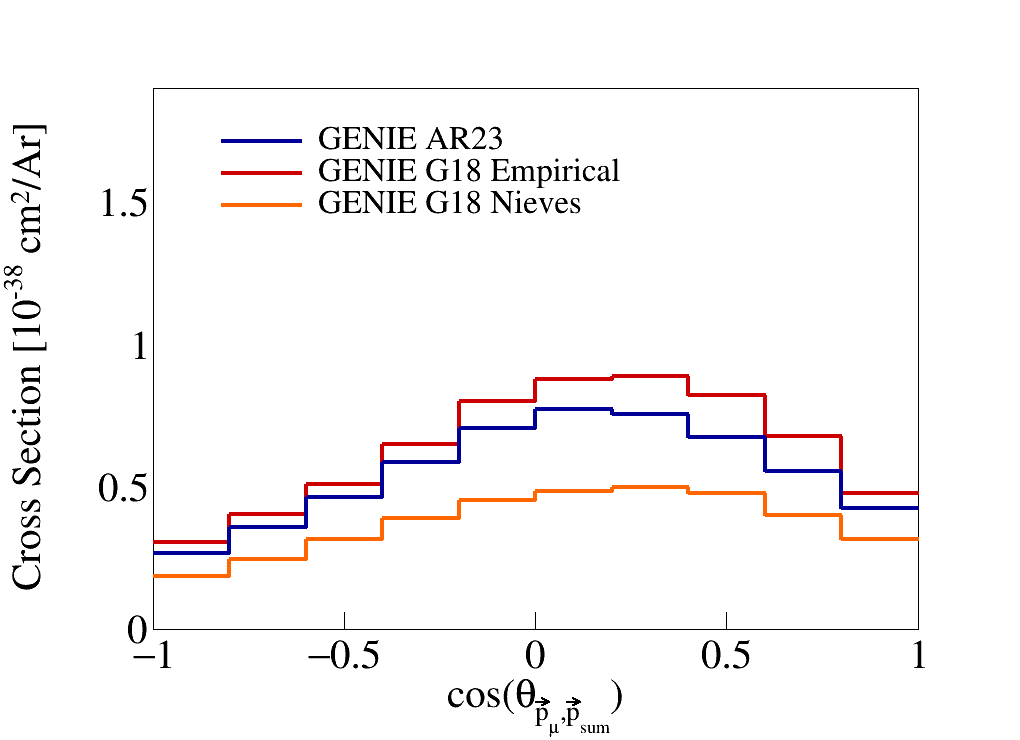
\includegraphics[width=3in]{Figs/Overlay/MEC/Overlay_TrueCosOpeningAngleMuonTotalProtonPlot.png}}
    \caption{Transverse kinematic variables for pure MEC events}
    \label{fig:transverse-k-mec}
\end{figure}

\begin{figure}
    \centering
    \subfloat{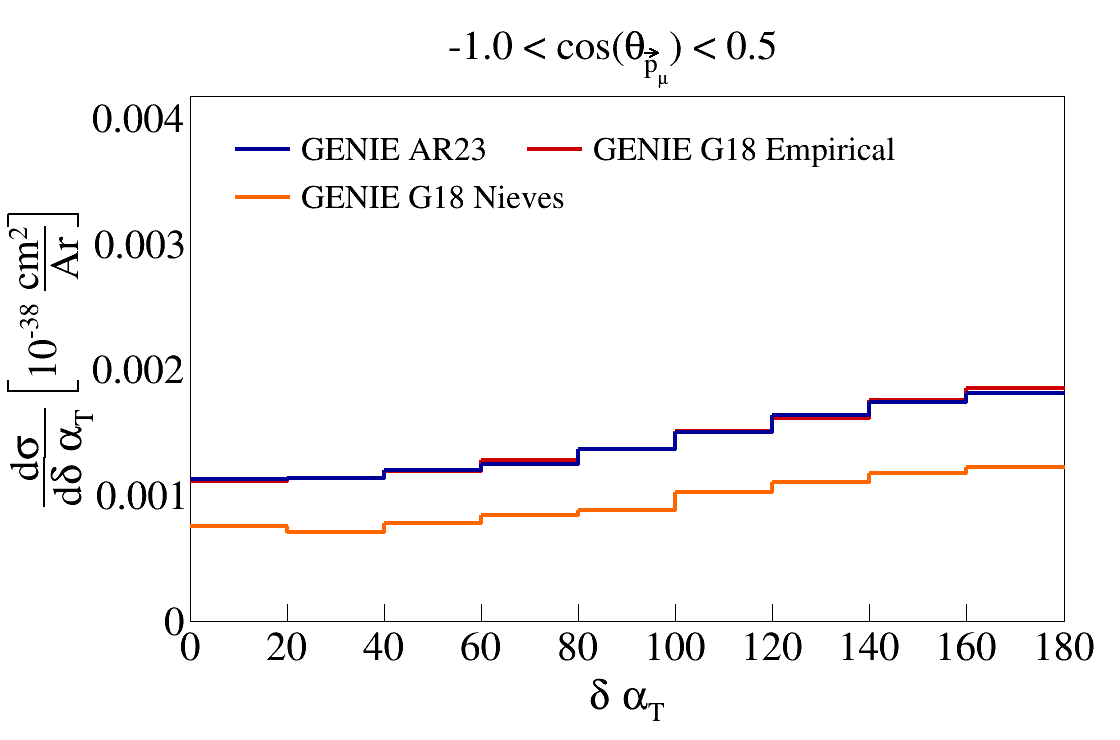
\includegraphics[width=3in]{Figs/Overlay/MEC/Serial/TrueSerialDeltaAlphaT_InMuonCosThetaPlot_0.png}}
    \subfloat{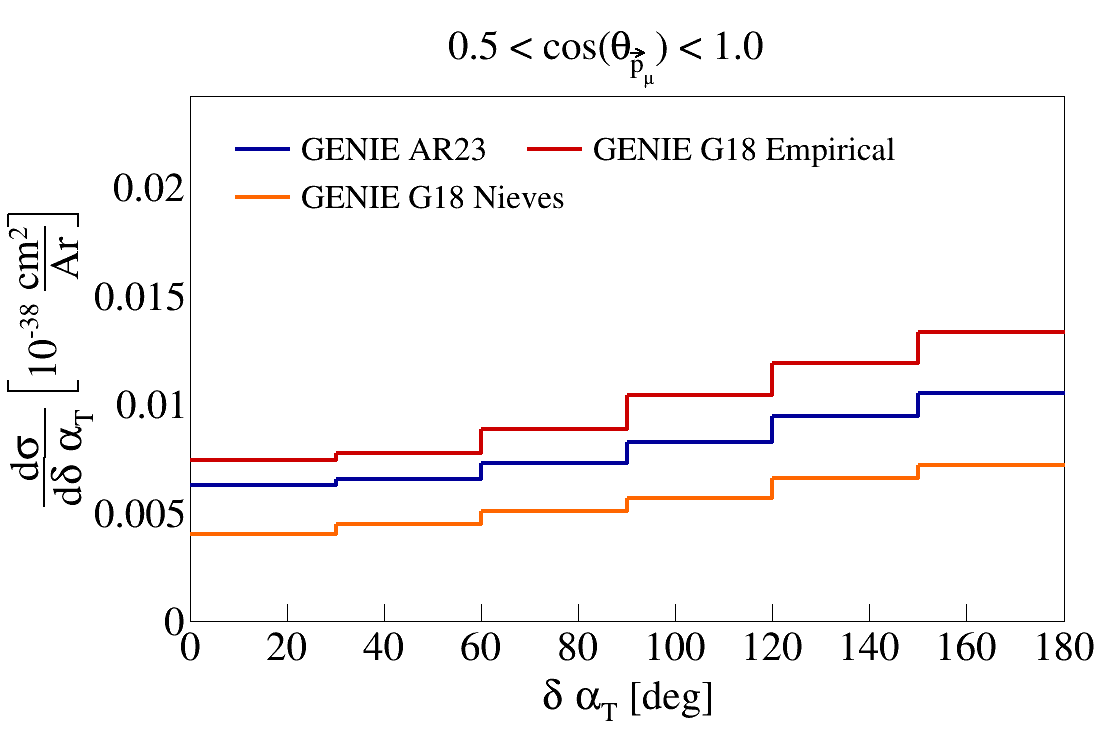
\includegraphics[width=3in]{Figs/Overlay/MEC/Serial/TrueSerialDeltaAlphaT_InMuonCosThetaPlot_1.png}} \\
    \subfloat{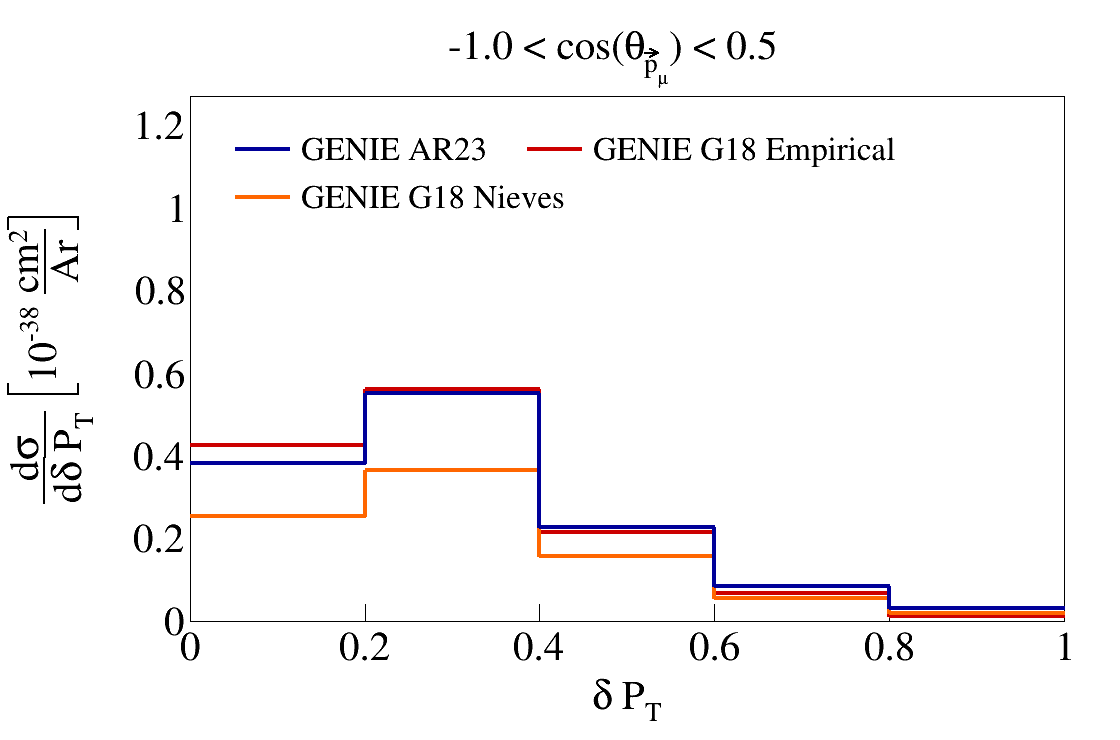
\includegraphics[width=3in]{Figs/Overlay/MEC/Serial/TrueSerialTransverseMomentum_InMuonCosThetaPlot_0.png}}
    \subfloat{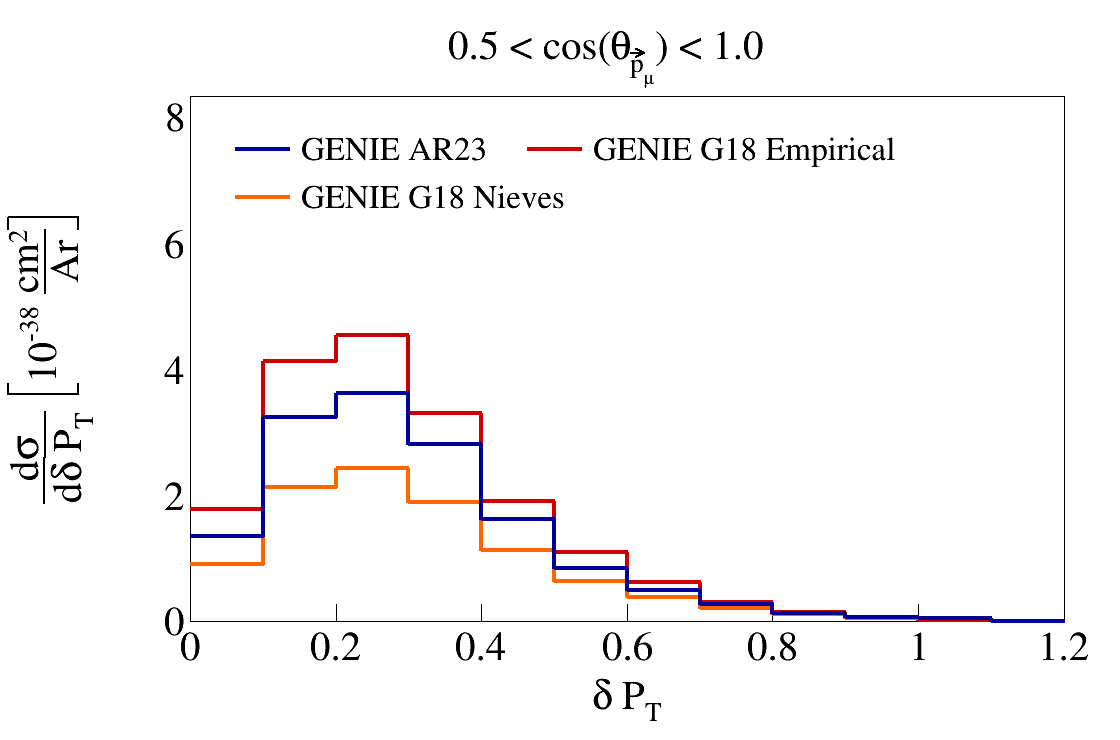
\includegraphics[width=3in]{Figs/Overlay/MEC/Serial/TrueSerialTransverseMomentum_InMuonCosThetaPlot_1.png}} \\
    \subfloat{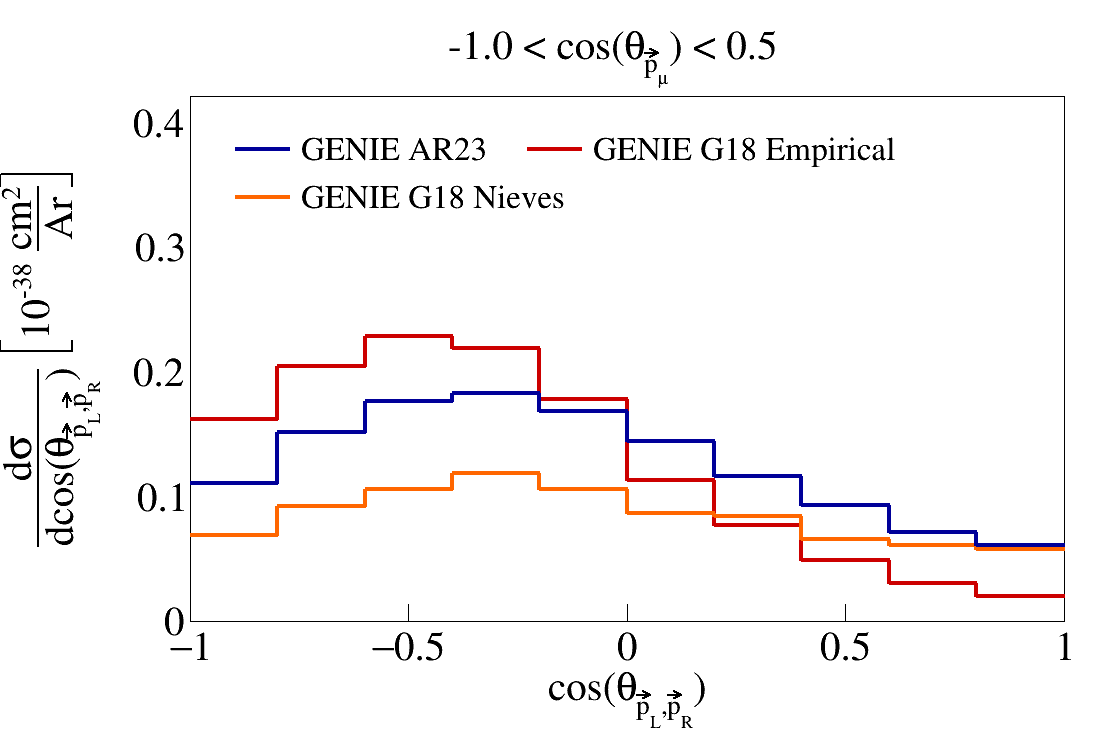
\includegraphics[width=3in]{Figs/Overlay/MEC/Serial/TrueSerialCosOpeningAngleProtons_InMuonCosThetaPlot_0.png}}
    \subfloat{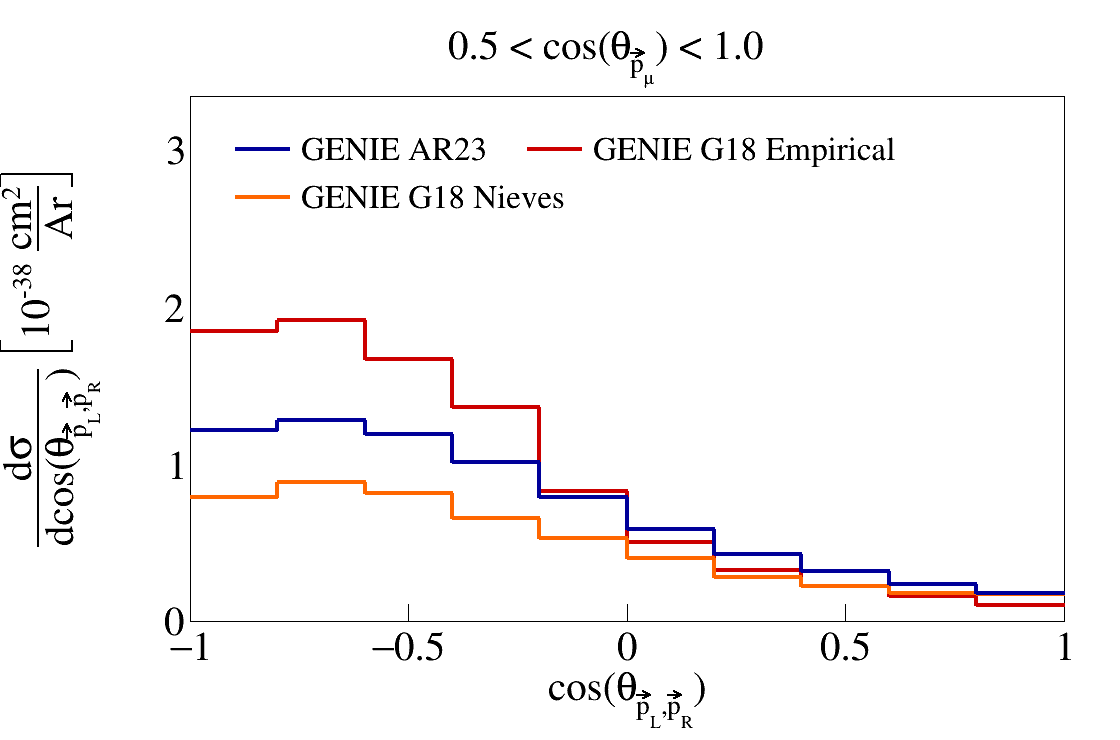
\includegraphics[width=3in]{Figs/Overlay/MEC/Serial/TrueSerialCosOpeningAngleProtons_InMuonCosThetaPlot_1.png}} \\
    \subfloat{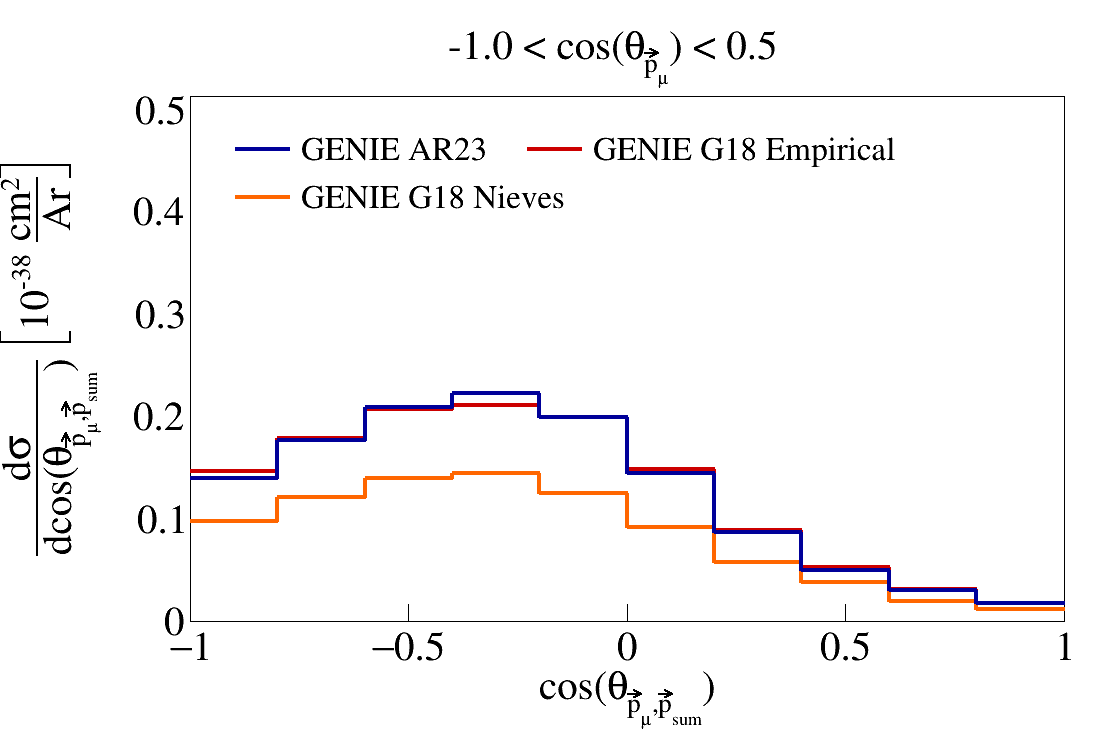
\includegraphics[width=3in]{Figs/Overlay/MEC/Serial/TrueSerialCosOpeningAngleMuonTotalProton_InMuonCosThetaPlot_0.png}}
    \subfloat{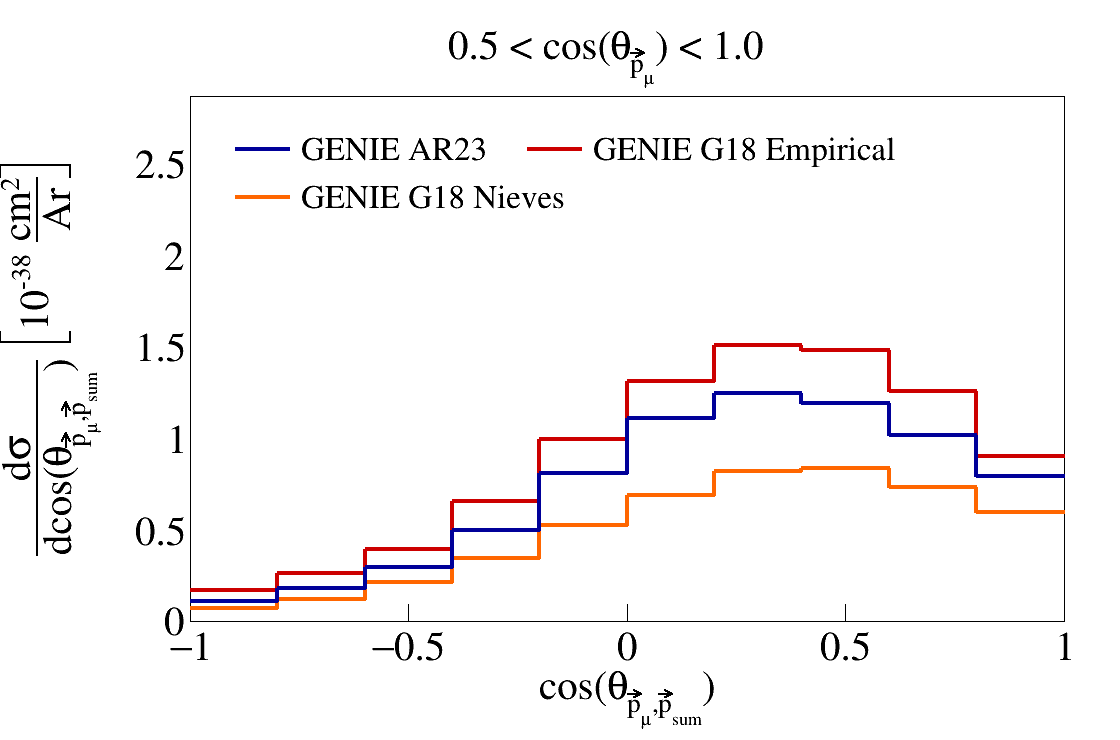
\includegraphics[width=3in]{Figs/Overlay/MEC/Serial/TrueSerialCosOpeningAngleMuonTotalProton_InMuonCosThetaPlot_1.png}} 
    \caption{Sliced double differential plots for pure MEC events}
    \label{fig:sliced-double-mec}
\end{figure}

\section{CAFAna analysis}

To perform analysis on experiment data, we will be using the CAFAna framework. This allows us to perform cuts based on the reconstructed and Monte Carlo data (if available, i.e., only in the case of dealing with simulated events), to discriminate events. To discriminate events based on their Monte Carlo data, we perform a simple \verb|TruthCut| that checks the following:
\begin{enumerate}[label=(\roman*)]
    \item That the neutrino interaction takes place in the fiducial volume
    \item That the neutrino is a muon neutrino
    \item That the interaction is a charged current interaction
    \item That the there is only one muon in our allowed momentum range
    \item That there are only two protons in our allowed momentum range
    \item That there are no charged/neutral pions in our defined momenta ranges
\end{enumerate}
Using the reconstructed event data, we can perform a \verb|Cut| that checks the following:
\begin{enumerate}[label=(\roman*)]
    \item The reconstructed vertex for the neutrino interaction takes place in the fiducial volume
    \item That the event is not a cosmic event by Pandora's criteria (using \verb|nu_score| to check how neutrino like the slice is, and \verb|fmatch.score| with \verb|fmatch.time| to check the event comes from the beam
    \item That there is one muon track with $L_{\text{track}} > 50$ cm, $\chi^2_\mu < 30$, $\chi^2_p > 60$, and this being the longest reconstructed track, and that this has momentum in our allowed range
    \item That there are two proton tracks with $\chi^2_p < 100$, and that these have momentum in our allowed range
    \item That there are no other reconstructed tracks with momentum in the allowed range for charged pions
    \item That there are no reconstructed particles with a positive \verb|trackScore| less than 0.5, so we don't allow any neutral pions
\end{enumerate}
Using these two discriminators on simulated events, the reconstructed events that satisfy the signal definition, and distinguish between true signal events and background events. This is shown in more detail for all our variables in the next section.

We use a one-bin histogram with lower bound $0$ and upper bound of $3$ in the true energy variable to get total counts of generated events, true signal events, all reconstructed events, and efficiency and purity data after each of the cuts we apply to the reconstructed events. These results are shown in Table~\ref{table:cut-efficiency-purity}. Counts are obtained using ROOT's command \verb|Histo->Integral()|. Global efficiency is defined as the ratio between events that pass the cut and reconstructed events, signal efficiency as the ratio between true events that pass the cut and the all true signal events, and purity as the ratio between true signal events that pass the cut and all events that pass the cut.

\begin{table}
    \begin{center}
        \begin{tabular}{|l|cccc|}
        \hline
        \textbf{Cut}         & \textbf{Number of events} & \textbf{Global efficiency} & \textbf{Signal efficiency} & \textbf{Purity} \\ \hline
        All                  & 308481  & -       & -       & -      \\
        True signal events   & 6040.06 & -       & -       & -      \\
        All reco events      & 175064  & 100\%   & -       & -      \\
        Cosmic cut           & 140772  & 80.41\% & 84.67\% & 3.63\% \\
        Vertex in FV cut     & 82953.4 & 47.39\% & 83.87\% & 6.11\% \\
        One muon cut         & 33951   & 19.39\% & 43.55\% & 7.75\% \\
        Two protons cut      & 2727.77 & 1.56\%  & 17.74\% & 39.29\% \\
        No charged pions cut & 1266.46 & 0.72\%  & 12.90\% & 61.54\% \\
        No neutral pions cut & 1120.33 & 0.64\%  & 12.10\% & 65.22\% \\ \hline
        \end{tabular}
    \end{center}
    \caption{Global efficiency, selection efficiency, and purity for cuts made in signal definition}
    \label{table:cut-efficiency-purity}
\end{table}

\section{SBND variable plots}

Using all the variable definitions as we did when studying the event generators, and the signal definition based on the cuts described in the previous section, we can generate plots for SBND data. The reconstructed single differential variables corresponding to vector opening angles and magnitudes are shown in Figure~\ref{fig:sbnd-vector-plots}. In these figures, three lines are shown, corresponding to: all reconstructed (all the reconstructed events that pass our signal definition), signal (reconstructed events that pass signal definition and are true signal events as determined by the \verb|TruthCut| from our previous section), and background (reconstructed events that pass signal definition but are not true signal events) events. Similarly, the variables relating multiple vectors are shown in Figure~\ref{fig:sbnd-opening-angles-transverse}, and double differential sliced variables are shown in Figure~\ref{fig:sbnd-double-diff-sliced}.

\begin{figure}
    \centering
    \subfloat{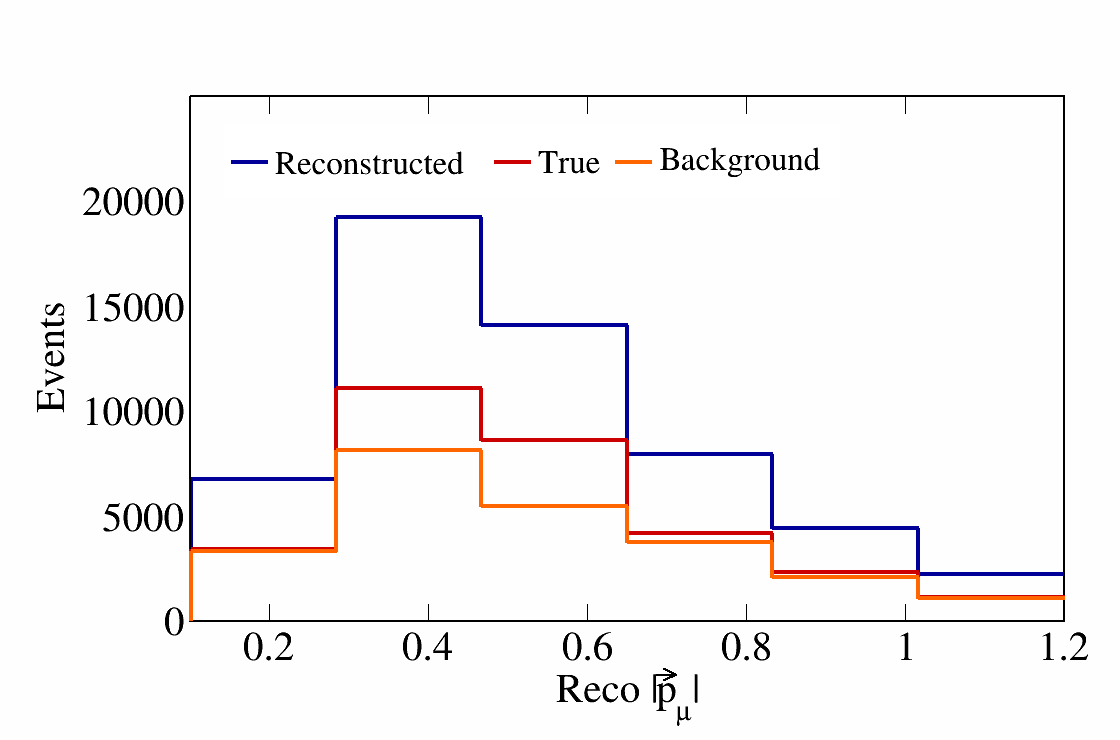
\includegraphics[width=3in]{Figs/CAFAna/MuonMomentum.png}}
    \subfloat{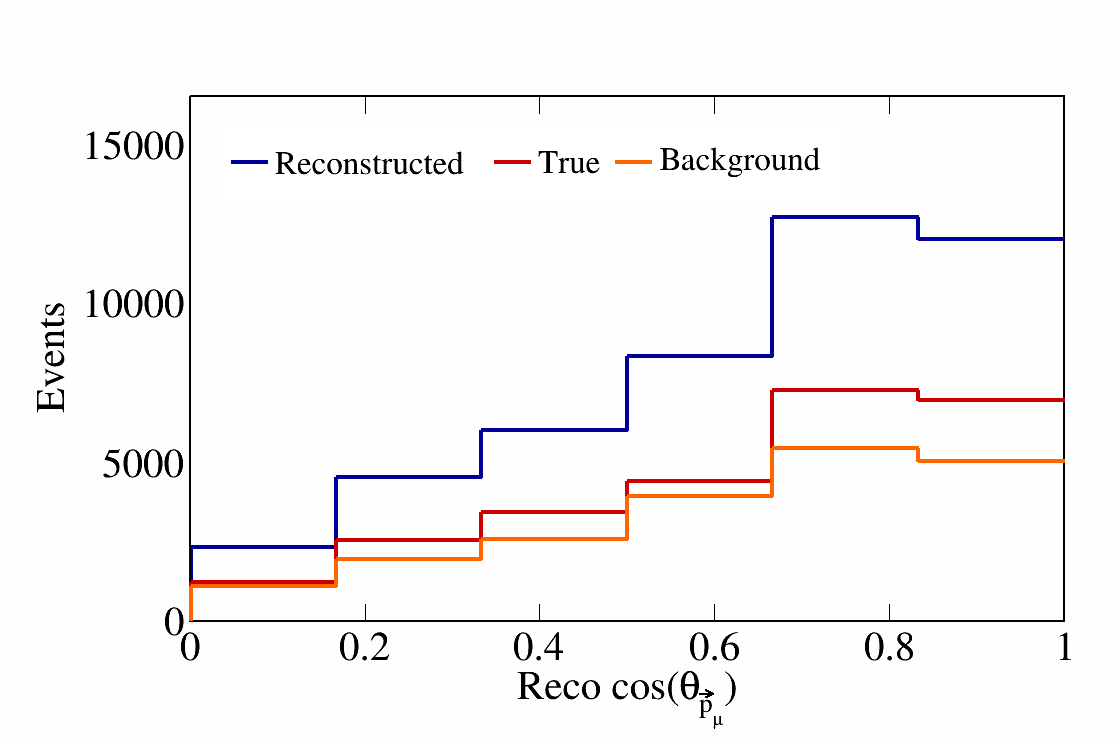
\includegraphics[width=3in]{Figs/CAFAna/MuonCosTheta.png}} \\
    \subfloat{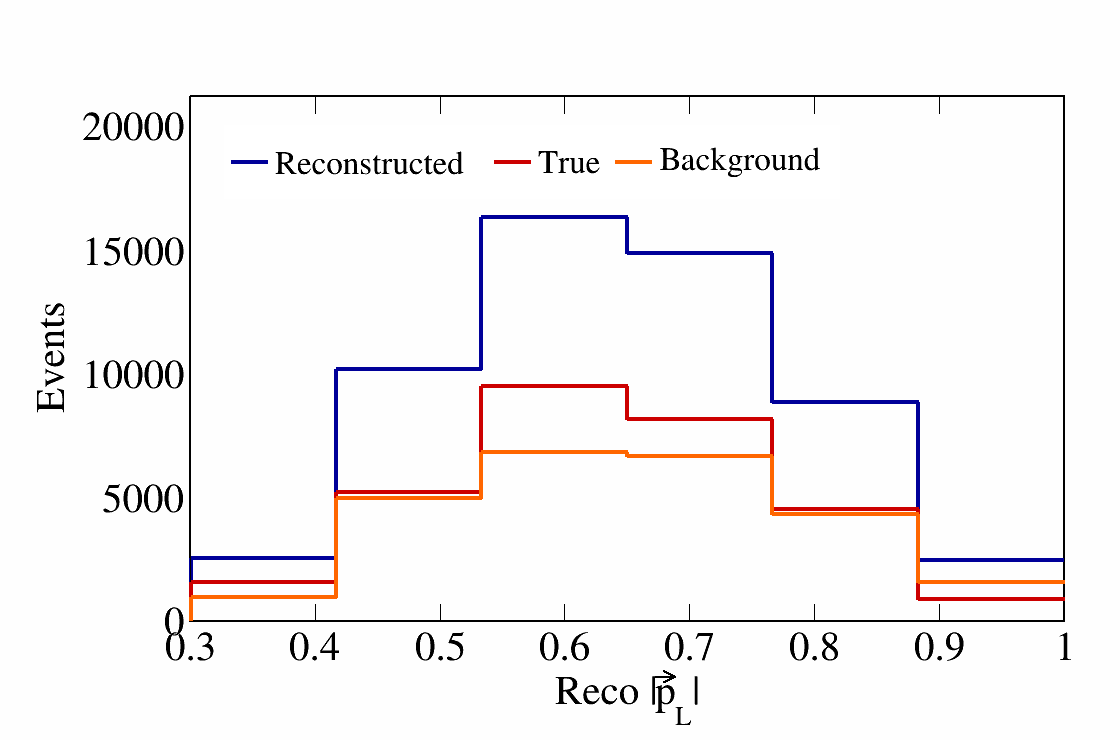
\includegraphics[width=3in]{Figs/CAFAna/LeadingProtonMomentum.png}}
    \subfloat{\includegraphics[width=3in]{Figs/CAFAna/LeadingProtonCosTheta.png}} \\
    \subfloat{\includegraphics[width=3in]{Figs/CAFAna/RecoilProtonMomentum.png}}
    \subfloat{\includegraphics[width=3in]{Figs/CAFAna/RecoilProtonCosTheta.png}} 
    \caption{Vector directions and magnitudes for SBND data}
    \label{fig:sbnd-vector-plots}
\end{figure}

\begin{figure}
    \centering
    \subfloat{\includegraphics[width=3in]{Figs/CAFAna/DeltaAlphaT.png}}
    \subfloat{\includegraphics[width=3in]{Figs/CAFAna/TransverseMomentum.png}} \\
    \subfloat{\includegraphics[width=3in]{Figs/CAFAna/CosOpeningAngleProtons.png}}
    \subfloat{\includegraphics[width=3in]{Figs/CAFAna/CosOpeningAngleMuonTotalProton.png}}
    \caption{Vector opening angles and transverse momentum for SBND data}
    \label{fig:sbnd-opening-angles-transverse}
\end{figure}

\begin{figure}
    \centering
    \subfloat{\includegraphics[width=3in]{Figs/CAFAna/Serial/SerialDeltaAlphaT_InMuonCosTheta_0.png}}
    \subfloat{\includegraphics[width=3in]{Figs/CAFAna/Serial/SerialDeltaAlphaT_InMuonCosTheta_1.png}} \\
    \subfloat{\includegraphics[width=3in]{Figs/CAFAna/Serial/SerialTransverseMomentum_InMuonCosTheta_0.png}}
    \subfloat{\includegraphics[width=3in]{Figs/CAFAna/Serial/SerialTransverseMomentum_InMuonCosTheta_1.png}} \\
    \subfloat{\includegraphics[width=3in]{Figs/CAFAna/Serial/SerialCosOpeningAngleProtons_InMuonCosTheta_0.png}}
    \subfloat{\includegraphics[width=3in]{Figs/CAFAna/Serial/SerialCosOpeningAngleProtons_InMuonCosTheta_1.png}} \\
    \subfloat{\includegraphics[width=3in]{Figs/CAFAna/Serial/SerialCosOpeningAngleMuonTotalProton_InMuonCosTheta_0.png}}
    \subfloat{\includegraphics[width=3in]{Figs/CAFAna/Serial/SerialCosOpeningAngleMuonTotalProton_InMuonCosTheta_1.png}}
    \caption{Sliced double differential plots for SBND events}
    \label{fig:sbnd-double-diff-sliced}
\end{figure}

\section{SBND signal efficiency}

Using the truth information about reconstructed events, we can also compute signal efficiency on a bin-by-bin basis. To be precise, signal definition on a bin \verb|i| is defined as the ratio between the number of events generated in bin \verb|i| and reconstructed in any bin over the number of events generated in bin \verb|i|. These plots are shown in Figure~\ref{fig:sbnd-signal-efficiency-vector-plots} and Figure~\ref{fig:sbnd-signal-efficiency-opening-angles-transverse} for single-differential variables and Figure~\ref{fig:sbnd-signal-efficiency-double-differential} for double differential variables.

\begin{figure}
    \centering
    \subfloat{\includegraphics[width=3in]{Figs/CAFAna/Efficiency/TruthMuonMomentum.png}}
    \subfloat{\includegraphics[width=3in]{Figs/CAFAna/Efficiency/TruthMuonCosTheta.png}} \\
    \subfloat{\includegraphics[width=3in]{Figs/CAFAna/Efficiency/TruthLeadingProtonMomentum.png}}
    \subfloat{\includegraphics[width=3in]{Figs/CAFAna/Efficiency/TruthLeadingProtonCosTheta.png}} \\
    \subfloat{\includegraphics[width=3in]{Figs/CAFAna/Efficiency/TruthRecoilProtonMomentum.png}}
    \subfloat{\includegraphics[width=3in]{Figs/CAFAna/Efficiency/TruthRecoilProtonCosTheta.png}} 
    \caption{Signal efficiency plots for single differential vector directions and magnitudes}
    \label{fig:sbnd-signal-efficiency-vector-plots}
\end{figure}

\begin{figure}
    \centering
    \subfloat{\includegraphics[width=3in]{Figs/CAFAna/Efficiency/TruthDeltaAlphaT.png}}
    \subfloat{\includegraphics[width=3in]{Figs/CAFAna/Efficiency/TruthTransverseMomentum.png}} \\
    \subfloat{\includegraphics[width=3in]{Figs/CAFAna/Efficiency/TruthCosOpeningAngleProtons.png}}
    \subfloat{\includegraphics[width=3in]{Figs/CAFAna/Efficiency/TruthCosOpeningAngleMuonTotalProton.png}}
    \caption{Signal efficiency plots for single differential vector opening angles and transverse momentum}
    \label{fig:sbnd-signal-efficiency-opening-angles-transverse}
\end{figure}

\begin{figure}
    \centering
    \subfloat{\includegraphics[width=3in]{Figs/CAFAna/Efficiency/TrueSerialDeltaAlphaT_InMuonCosTheta_0.png}}
    \subfloat{\includegraphics[width=3in]{Figs/CAFAna/Efficiency/TrueSerialDeltaAlphaT_InMuonCosTheta_1.png}} \\
    \subfloat{\includegraphics[width=3in]{Figs/CAFAna/Efficiency/TrueSerialTransverseMomentum_InMuonCosTheta_0.png}}
    \subfloat{\includegraphics[width=3in]{Figs/CAFAna/Efficiency/TrueSerialTransverseMomentum_InMuonCosTheta_1.png}} \\
    \subfloat{\includegraphics[width=3in]{Figs/CAFAna/Efficiency/TrueSerialCosOpeningAngleProtons_InMuonCosTheta_0.png}}
    \subfloat{\includegraphics[width=3in]{Figs/CAFAna/Efficiency/TrueSerialCosOpeningAngleProtons_InMuonCosTheta_1.png}} \\
    \subfloat{\includegraphics[width=3in]{Figs/CAFAna/Efficiency/TrueSerialCosOpeningAngleMuonTotalProton_InMuonCosTheta_0.png}}
    \subfloat{\includegraphics[width=3in]{Figs/CAFAna/Efficiency/TrueSerialCosOpeningAngleMuonTotalProton_InMuonCosTheta_1.png}}
    \caption{Signal efficiency plots for double differential variables}
    \label{fig:sbnd-signal-efficiency-double-differential}
\end{figure}

\section{SBND migration and response matrices}

Further, we compute migration matrices which give us a measure of how reliable our reconstructed variables are. A given column in this matrix represents a bin of the truth variable, i.e., the value with which the event was generated. Then, each row corresponds to a reconstructed bin of the same variable, and each cell corresponds to the probability that an event generated with the truth value corresponding to the column gets reconstructed with the value corresponding to the row. For the migration matrix, we consider true signal events that were reconstructed and satisfy our signal definition in the denominator. Therefore, the values in each column must add up to $1$. The migration matrices for the single differential variables are presented in Figure~\ref{fig:migration-vector-plots} and Figure~\ref{fig:migration-opening-angles-transverse}. The migration matrices for the double differential variables (given in terms of the bin number) are presented in Figure~\ref{fig:migration-double-differential}.

Response matrices are computed in a similar manner, but using the total number of generated events in the denominator when computing the ratios, i.e., without requiring the events to be successfully reconstructed. Therefore, for these matrices, the columns of the response matrices do not have to add up to $1$. The response matrices for single differential variables are presented in Figure~\ref{fig:response-vector-plots} and Figure~\ref{fig:response-opening-angles-transverse}, and the double differential response matrices are given in Figure~\ref{fig:response-double-differential}.

\begin{figure}
    \centering
    \subfloat{\includegraphics[width=3.25in]{Figs/CAFAna/Matrices/MigrationMuonMomentum.png}}
    \subfloat{\includegraphics[width=3.25in]{Figs/CAFAna/Matrices/MigrationMuonCosTheta.png}} \\
    \subfloat{\includegraphics[width=3.25in]{Figs/CAFAna/Matrices/MigrationLeadingProtonMomentum.png}}
    \subfloat{\includegraphics[width=3.25in]{Figs/CAFAna/Matrices/MigrationLeadingProtonCosTheta.png}} \\
    \subfloat{\includegraphics[width=3.25in]{Figs/CAFAna/Matrices/MigrationRecoilProtonMomentum.png}}
    \subfloat{\includegraphics[width=3.25in]{Figs/CAFAna/Matrices/MigrationRecoilProtonCosTheta.png}}
    \caption{Migration matrices for signal differential vector directions and magnitudes}
    \label{fig:migration-vector-plots}
\end{figure}

\begin{figure}
    \centering
    \subfloat{\includegraphics[width=3.25in]{Figs/CAFAna/Matrices/MigrationDeltaAlphaT.png}}
    \subfloat{\includegraphics[width=3.25in]{Figs/CAFAna/Matrices/MigrationTransverseMomentum.png}} \\
    \subfloat{\includegraphics[width=3.25in]{Figs/CAFAna/Matrices/MigrationCosOpeningAngleProtons.png}}
    \subfloat{\includegraphics[width=3.25in]{Figs/CAFAna/Matrices/MigrationCosOpeningAngleMuonTotalProton.png}}
    \caption{Migration matrices for signal differential vector opening angles and transverse momentum}
    \label{fig:migration-opening-angles-transverse}
\end{figure}

\begin{figure}
    \centering
    \subfloat{\includegraphics[width=3.25in]{Figs/CAFAna/Matrices/MigrationSerialDeltaAlphaT_InMuonCosTheta.png}}
    \subfloat{\includegraphics[width=3.25in]{Figs/CAFAna/Matrices/MigrationSerialTransverseMomentum_InMuonCosTheta.png}} \\
    \subfloat{\includegraphics[width=3.25in]{Figs/CAFAna/Matrices/MigrationSerialCosOpeningAngleProtons_InMuonCosTheta.png}}
    \subfloat{\includegraphics[width=3.25in]{Figs/CAFAna/Matrices/MigrationSerialCosOpeningAngleMuonTotalProton_InMuonCosTheta.png}}
    \caption{Migration matrices for double differential variables}
    \label{fig:migration-double-differential}
\end{figure}

\begin{figure}
    \centering
    \subfloat{\includegraphics[width=3.25in]{Figs/CAFAna/Matrices/ResponseMuonMomentum.png}}
    \subfloat{\includegraphics[width=3.25in]{Figs/CAFAna/Matrices/ResponseMuonCosTheta.png}} \\
    \subfloat{\includegraphics[width=3.25in]{Figs/CAFAna/Matrices/ResponseLeadingProtonMomentum.png}}
    \subfloat{\includegraphics[width=3.25in]{Figs/CAFAna/Matrices/ResponseLeadingProtonCosTheta.png}} \\
    \subfloat{\includegraphics[width=3.25in]{Figs/CAFAna/Matrices/ResponseRecoilProtonMomentum.png}}
    \subfloat{\includegraphics[width=3.25in]{Figs/CAFAna/Matrices/ResponseRecoilProtonCosTheta.png}}
    \caption{Response matrices for signal differential vector directions and magnitudes}
    \label{fig:response-vector-plots}
\end{figure}

\begin{figure}
    \centering
    \subfloat{\includegraphics[width=3.25in]{Figs/CAFAna/Matrices/ResponseDeltaAlphaT.png}}
    \subfloat{\includegraphics[width=3.25in]{Figs/CAFAna/Matrices/ResponseTransverseMomentum.png}} \\
    \subfloat{\includegraphics[width=3.25in]{Figs/CAFAna/Matrices/ResponseCosOpeningAngleProtons.png}}
    \subfloat{\includegraphics[width=3.25in]{Figs/CAFAna/Matrices/ResponseCosOpeningAngleMuonTotalProton.png}}
    \caption{Response matrices for signal differential vector opening angles and transverse momentum}
    \label{fig:response-opening-angles-transverse}
\end{figure}

\begin{figure}
    \centering
    \subfloat{\includegraphics[width=3.25in]{Figs/CAFAna/Matrices/ResponseSerialDeltaAlphaT_InMuonCosTheta.png}}
    \subfloat{\includegraphics[width=3.25in]{Figs/CAFAna/Matrices/ResponseSerialTransverseMomentum_InMuonCosTheta.png}} \\
    \subfloat{\includegraphics[width=3.25in]{Figs/CAFAna/Matrices/ResponseSerialCosOpeningAngleProtons_InMuonCosTheta.png}}
    \subfloat{\includegraphics[width=3.25in]{Figs/CAFAna/Matrices/ResponseSerialCosOpeningAngleMuonTotalProton_InMuonCosTheta.png}}
    \caption{Response matrices for double differential variables}
    \label{fig:response-double-differential}
\end{figure}

\end{document}
